\documentclass[twoside]{styles/uocthesis}

\usepackage{subcaption}
\captionsetup{compatibility=false}


\usepackage[pdftex]{graphicx} %Loading the package
\graphicspath{{figures/}} %Setting the 


\usepackage[acronym]{glossaries}
\usepackage{booktabs}
\usepackage{styles/gnuplot-lua-tikz}
\usepackage{tikz}
\usepackage{amsmath}
\usepackage{enumitem}




\Title{Interactive Machine Learning for Object Detection and Instance Recognition}
\Author{Oliver Batchelor}
\Year{2018}

\Supervisor{Prof. Richard Green}
\Department{Department of Computer Science}

\makeglossaries




\begin{document}

\prelimpages


\titlepage


\abstract{%
TODO

}

\tableofcontents



\printglossaries

\newacronym{FCN}{FCN}{Fully Convolutional Network}
\newacronym{IOU}{IOU}{Intersection Over Union}
\newacronym{VOC}{VOC}{Visual Object Classes}
\newacronym{mIOU}{mIOU}{mean Intersection Over Union}
\newacronym{AMT}{AMT}{Amazon Mechanical Turk}
\newacronym{NLL}{NLL}{Negative Loss Likelihood}
\newacronym{CRF}{CRF}{Conditional Random Field}

\newacronym{CNN}{CNN}{Convolutional Neural Netowork}
\newacronym{MCDNN}{MCDNN}{Multi Column Deep Neural Network}

\newacronym{SIFT}{SIFT}{Scale Invariant Feature Transform}
\newacronym{SURF}{SURF}{Speeded Up Robust Features}

\newacronym{ALOI}{ALOI}{Amsterdam Library of Images}
\newacronym{MSR}{MSR}{Microsoft Research}

\newacronym{BOW}{BoW}{Bag of Words}
\newacronym{BOVW}{BoVW}{Bag of Visual Words}

\newacronym{ANN}{ANN}{Approximate Nearest Neighbor}
\newacronym{SGD}{SGD}{Stochastic Gradient Descent}
\newacronym{ASGD}{ASGD}{Asynchronous Stochastic Gradient Descent}
\newacronym{LOO}{LOO}{Leave One Out}

\newacronym{NCA}{NCA}{Neighborhood Components Analysis}
\newacronym{MEGM}{MEGM}{Mean square Error's Gradient Minimization}

\newacronym{KNN}{kNN}{k-Nearest Neighbor}

\newacronym{MSE}{MSE}{Mean Squared Error}
\newacronym{LMNN}{LMNN}{Large Margin Nearest Neighbor}
\newacronym{SVM}{SVM}{Support Vector Machine}

\newacronym{PCA}{PCA}{Principle Components Analysis}
\newacronym{DRLIM}{DrLIM}{Dimensionality Reduction by Learning an Invariant Mapping}
 
\newacronym{GPU}{GPU}{Graphics Processing Unit}


\acknowledgments{%
I will like to thank all the hedgehogs, without there help this
thesis would not be a reality.}

\textpages




\chapter{Bootstrap}
 

Applying deep learning to new domains usually implies a considerable data collection problem. We look at idea of how we can use a partially trained model as an aid to a human annotator. We do this by providing the partially trained model's prediction as a starting point for a human annotator to directly edit. This is demonstrated by applying our ideas to building a small segmentation dataset for labeling trees in a plantation. We also show that by starting with a pre--trained model and fine--tuning, we can provide a useful aid to a human annotator using very few input images.


\section {Introduction}


One of the greatest problems faced in machine learning is obtaining accurate and sufficient annotated data where typically thousands of examples are required. Deep learning has been shown to perform well on large datasets, and there exists a variety of large datasets in the public domain for research purposes. Applying deep learning to a new application presents a data collection and annotation problem, for which there are a number of active research topics such as active learning, semi-supervised learning, and interactive machine learning. We discuss these topics in more detail below.

Not only is it necessary to collect and annotate data - one of the primary questions asked when considering the use of machine learning is 'How many examples are necessary?'. To which the usual answer is to by experimental validation where part of the data is held back and used to test the effectiveness of training on the other part.

We present a bootstrapping method for creating a segmentation dataset guided by a feedback loop using a human annotator and a model (a \gls{CNN}). We use segmentation as our task because it is applicable to many domains and is very flexible, for example, labelling tree branches using axis aligned bounding boxes is in-feasible. Our approach is based on using a partially trained model to assist the human annotator.

We show that by using transfer learning by fine tuning a pre--trained model, very few hand annotated images are necessary to provide a good level of assistance to a human annotator, using the related idea that recognition is better than recall. Just as it is much faster to recognise a solution rather than recall one from memory, if a model can produce an annotation which is mostly correct - a human can recognise and fix small problems much faster than reproducing the annotation from scratch. At worst the human annotator can discard the automatic solution and produce the annotation by hand, and learn a measure of the model's current level.

\begin{figure}[h]
\centering
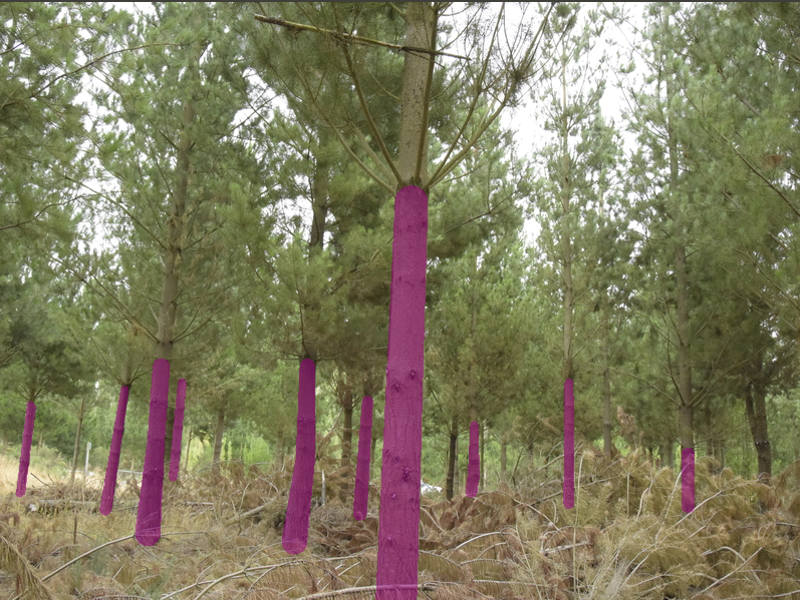
\includegraphics[width=0.9\linewidth]{bootstrap/trees_example.png}

\caption{Example from the trees dataset}
\label{fig:tree}
\end{figure}

\subsection{Related methods}


Human time becomes the main expense when annotating data, so in order to minimise cost there exist strategies such as crowd sourcing. In order to get a lot of people to contribute there exist methods such as gamification, e.g. a game Quick Draw \cite{Ha2017}, or presenting the task as proof of human--ness \cite{Goodfellow2013a}.  Most annotations performed on a large scale rely on brute labour, with many using global markets such as \gls{AMT}. Large scale datasets such as ImageNet \cite{Russakovsky2015} are built with \gls{AMT}. 

The closest related work to ours we have found, with a very similar idea is \cite{Papadopoulos2016}. Instead of annotating a dataset from scratch - they iteratively improve a partially trained model by asking questions of a human annotator. They initially bootstrap a model using semi-supervised methods with per--image labels. A simple Yes/No questioning process is then used used to annotate a dataset by refining bounding boxes proposed by the model (and intelligently prune bounding box proposals by adjusting thresholds and overlap \gls{IOU}). They report the speedup to achieve nearly equivalent accuracy of $6\times$ to $9\times$.

A closely related research area is active learning. The motto of active learning is ``putting the model in the loop'' (or conversely the human, depending on the perspective). Active learning requires a model with some estimate of uncertainty. Given a pool of non annotated examples, an algorithm can choose which examples require human annotation (because the model is uncertain), or go with the model's annotation (because the model is certain). One recent example, using active learning for segmentation is \cite{Xu2017}, where they focus on finding the nodes (super pixels) which induce the largest change in a \gls{CRF} model .

Semi-supervised machine learning attempts to use existing knowledge or domain properties to infer annotations. For example using motion cues to give indications of object boundaries \cite{Hong2017}, or using an image classifier to perform object detection by blanking out portions of the image, so as to determine which parts are important \cite{Bazzani2016}. Semi-supervised methods often substitute for human labour, but in doing so make sacrifices of the quality and often result in somewhat noisy data. As a result semi-supervised methods are often used as a means of bootstrapping a model before involving a human annotator, for example as used in \cite{Papadopoulos2016}.


\subsection {Assisted annotation}


\begin{figure}[ht]
\centering
\begin{subfigure}{.25\textwidth}
  \centering
  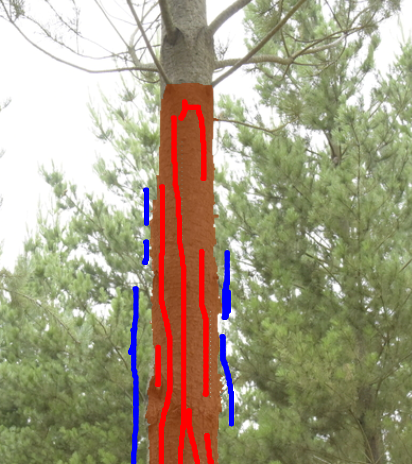
\includegraphics[width=0.5\linewidth]{bootstrap/labelme.png}
  \caption{Labelme mask annotation}  
  \label{fig:labelme}
\end{subfigure}%
\begin{subfigure}{.25\textwidth}
  \centering
  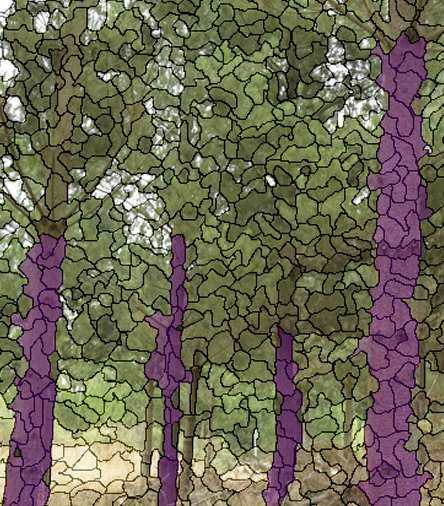
\includegraphics[width=.5\linewidth]{bootstrap/superpixels.png}
  \caption{Annotation using super pixels}
  \label{fig:superpixels}
\end{subfigure}

\caption{Assisted annotation methods}
\label{fig:annot_method}
\end{figure}


In our initial attempts to annotate a dataset, one of the problems was often that using the assisted annotation tools such as the mask tool in the LabelMe \cite{Russell2007} interface actually required more work than manually annotating the polygon boundary from scratch. The LabelMe mask tool provides a GrabCut--esque interface where positive and negative stripes can be painted onto an image. Our experience in creating a mask for a tree trunk can be seen in Figure \ref{fig:labelme} where annotations are bright red and green. The initial painted stripe provided a rough outline, but many small annotations were needed to make the mask resemble the true edge of the tree trunk.

In \cite{Galloway2017}, the images are segmented using superpixels (clusters of pixels grouped with an unsupervised algorithm), where labelling groups of pixels is substantially less work than labelling individual pixels, and superpixels seem to do well at finding image boundaries where \gls{CNN} are often imprecise. This does present some difficulties, such as the ambiguity where multiple classes are covered in one superpixel. In our experiences using superpixels provided imprecise boundaries and saved little time, an example of our tool with superpixel selection is shown in Figure \ref{fig:superpixels}.

Deep learning has previously been used to aid in object instance selection. In \cite{Xu2016} a \gls{FCN} is trained to perform semantic segmentation of objects in images as selected by users. Users click on an object (providing positive and negative points), which are passed to the model as distance maps along with the regular colour image data. Another recent approach is that of \cite{Xu2017} which also aims at interactive instance segmentation, using a rectangle as an input (also using a distance map), and producing an instance segmentation.

% \begin{figure*}[!ht]
% \centering

% \end{figure*}




\section{Proposed Method}

Our approach is to annotate data and train a model as we go. First annotate a small number of examples to begin with to create an initial training set, and use these examples to train an initial model. New examples are then classified by the model, at which point the human annotator fixes any mistakes and the corrected example is added to the training set. Initially the annotator will need to fix the majority of the data, and as the model improves such feedback will be required less and less. The idea is that the model will quickly learn the easy cases, which can be quickly ignored to save work, and the annotator will be left to invervene only with the more important challenging cases.

We have used this method to build a small scale tree trunk segmentation dataset, a prototype for the purposes of an automated drone tree pruning project for the purpose of pruning lower branches off young Pinus Radiata tree plantations. Our work is intended to allow the drone see the trees despite the forest. To evaluate methods of dataset construction and evaluate methods of annotation, we wrote an annotation application written with a Qt interface, with tools for drawing on masks and iterating the dataset and refining model proposed annotations.

Our workflow after first training some initial number of examples was to leave a training process in the background which would pick up newly created annotations after each training epoch. 


\subsection {Models}

\begin{figure}[h]
  \centering
  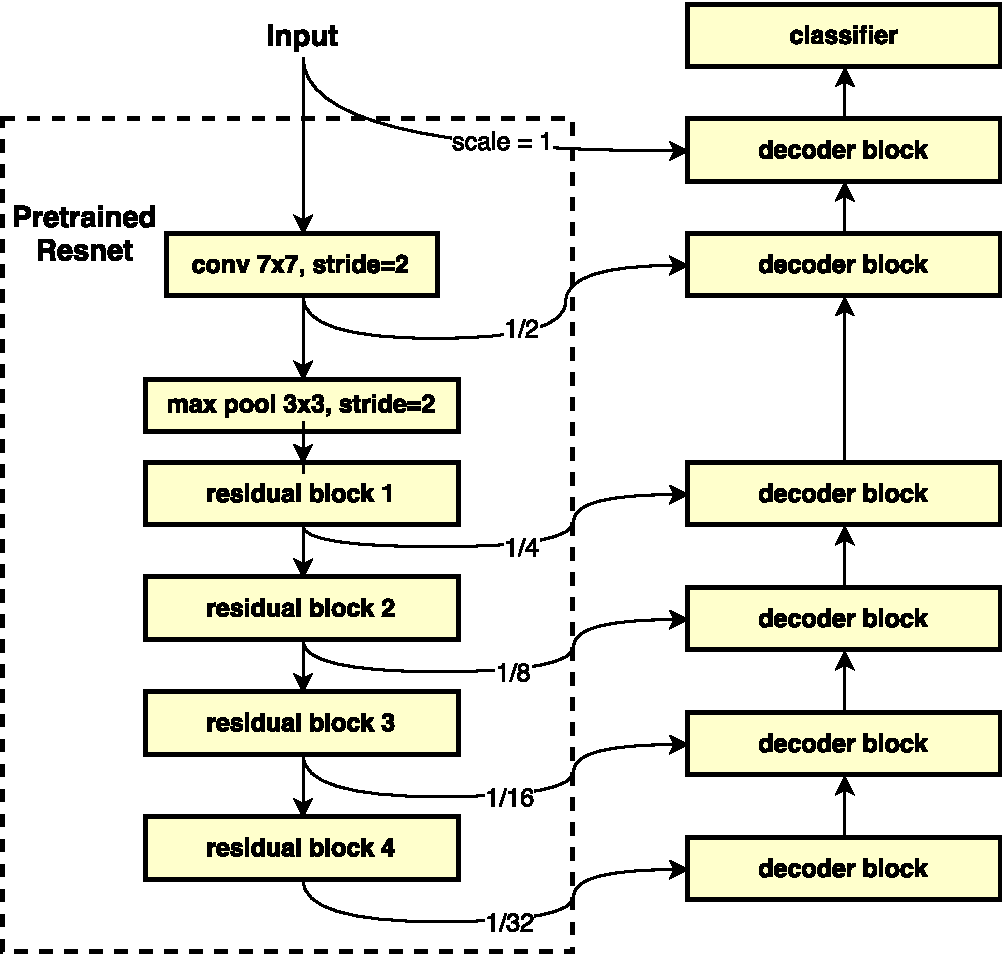
\includegraphics[width=0.9\linewidth]{bootstrap/network.pdf}
  \caption{Encoder--decoder network with pre-trained Resnet}  
  \label{fig:network}
\end{figure}
\begin{figure}
  \centering
  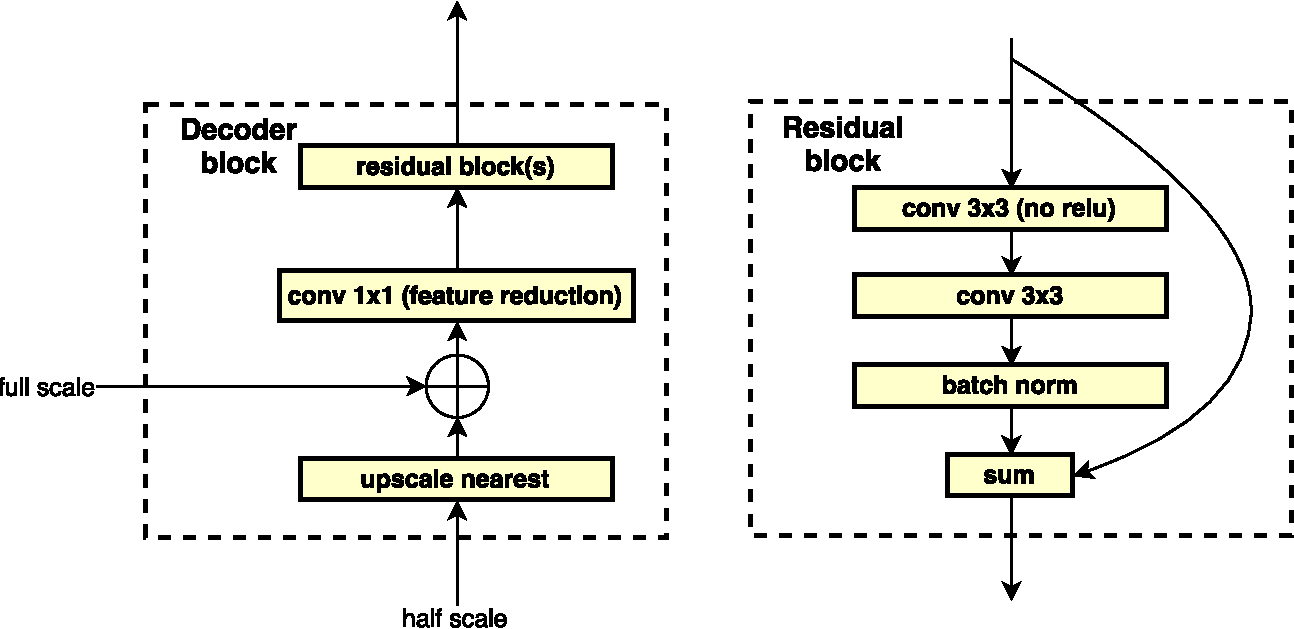
\includegraphics[width=0.9\linewidth]{bootstrap/network_blocks.pdf}
  \caption{Block sub networks}  
  \label{fig:decode_block}
\end{figure}

For our image segmentation model we have used an encoder--decoder with skip connections similar to UNet \cite{Ronneberger2015} (utilizing padding and without cropping the skip connections). Each level of the encoder and decoder (at the same resolution) are connected by a skip connection bypassing the lower layers of the network. We focus on two architectures, the first is a pre-trained ResNet model as an encoder with a decoder added, and the second is a symmetrical encoder and decoder. We refer to the first as ``pre-trained and the second as ``ladder'' in the experiments below.

The architecture based on the pre-trained ResNet is shown in Figure \ref{fig:network}, with the decoder and residual block used shown in Figure \ref{fig:decode_block}. The particular ResNet we use is the ``resnet18'' from the Pytorch model zoo, (the smallest of the various ResNet architectures) with weights trained on the ImageNet dataset. 

Our decoder for the ``pre-trained model uses a single residual block at the point labelled ``residual block(s)'' in Figure \ref{fig:decode_block}. The ``ladder'' model uses residual blocks of size (1, 2, 3, 3, 3, 3) in both encoder and decoder. Our decoder uses $ 1x1 $ convolutions to reduce the feature sizes coming from intermediate layers of the ResNet, the number of features used in the decoder is 16, with 8 additional features at each layer further down. An implicit Batch Normalisation layer and ReLU is present before every convolution.

Of note the first skip connection is directly the image input, and the second is directly after the $7x7, stride=2$ first convolution used by the ResNet.


\section {Experiments}


\subsection {Loss Function}


We primarily use the \gls{IOU} as a measure of comparison for segmentation. The \gls{IOU} is presented in Equation \ref{eq:iou} with $ A $ and $ B $ being sets. When training a model, we optimise the Jaccard Distance as a continuous approximation to the \gls{IOU}. This is shown in Equation \ref{eq:jaccard} where $ P $ is a binary prediction vector, which are image pixels output from the model and normalised using a sigmoid vector to be between 0 and 1. $ T $ is the binary target vector. Multiplication in these equations is element wise vector multiplication.


\begin{equation}
IOU = \frac{A \cap B}{A \cup B}
\label{eq:iou}
\end{equation}


\begin{equation}
Jacc = 1 - \frac{| PT |}{| P^2 | + | T^2 | - | PT |}
\label{eq:jaccard}
\end{equation}



\subsection {Image preparation}

We use images of a fixed size in order to train our network (for the purposes of processing images in batches), however because our network is a fully convolutional network we can then test on images of variable size. We show the effect of this processing later, as compared to training with full size images with batches of size one.

Data augmentation is used to add variety. We use random scales (0.8 to 1.25), crops and rotations (-5 to 5 degrees). We adjust colours on a per colour channel basis ($ \gamma = 0.9 $ to $ \gamma=1.1 $ )  $ x_a = x^{\gamma} $.

After scaling and rotation, we then crop an area of the image of $440 \times 440$ pixels (the original image size in the trees dataset is $800 \times 600$, down-scaled from the original photos of approximately 25 megapixels.

We employ image whitening as a last step, subtracting an approximate global mean (r, g, b) $ (0.485. 0.456, 0.406) $ and dividing by standard deviation $ (0.229, 0.224, 0.225) $ as to ensure consistency with the pre-processing used in ImageNet training with the pre--trained model.



\subsection {Datasets}




We developed a small scale dataset for segmentation of tree trunks in Pinus Radiata forests (using the approach described). The dataset consisting of 120 images each containing multiple instances of tree trunk. We labelled the most distinct instances in each image, where some images contained hundreds of background trees. Of the 120 images, we used 30 images for a validation set for the purposes of experimentation in this paper which were not used for training.

Along with our tree dataset, we've used classes from the Pascal VOC dataset in some experiments. We train with a mix of images from MS COCO \cite{Lin2014} training set along with the Pascal VOC 2012 training set, and use the VOC validation set for validation. The tree images typically contain more instances per image at higher resolution, but significantly less images than VOC and COCO images for each category.


\subsection {Minimum viable examples}

The effectiveness of involving the model early in the process will be determined by the point where fixing errors in the model's predictions becomes faster than simply annotating the image from scratch. The effect of number of examples was studied in \cite{Soekhoe} in the context of transfer learning. One finding was that with smaller numbers of examples, fixing the weights of earlier layers boosted performance when using less training examples.

We performed a simple validation experiment to investigate the effect of using less examples. The results can be seen in Figure \ref{fig:limited}, in each case the stated IOU is an average over several trials (the number can be seen in table \ref{fig:limit_params}, and is additionally averaged over the last 3 epochs of training. Here we have used classes from the Pascal VOC 2012 for comparison.

We can see that even for as few as 10 examples, the validation accuracy is not far off using a full dataset (1000s of images) in each case, and the difference between using 100 images and the full dataset in each case was very small. We expected to see the pre-trained model perform much better with a limited number of examples, as it does - however it seems to perform much better in the general case as well. The case matching our expectations is with the (much more limited) trees dataset.


\begin{table}[ht]
  \centering
    \caption{Training parameters for limited examples experiment}

%\noindent\resizebox{0.5\textwidth}{!}
\label{fig:limit_params}
\end{table}



\begin{figure}[ht]
\centering
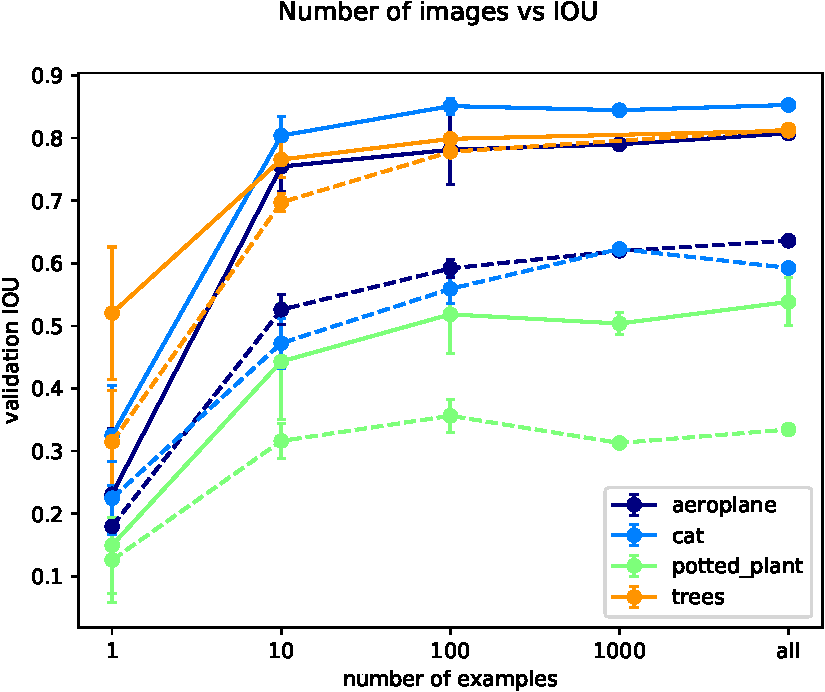
\includegraphics[width=0.9\linewidth]{bootstrap/limit.pdf}
\caption{Validation with a limited number of images, solid line is with the pre-trained model}  
\label{fig:limited}
\end{figure}



\subsection{Model fine-tuning}

We examined the best parameters for fine tuning, finding that allowing a small learning rate on the pre-trained model was advantageous. The effects can be seen in Figure \ref{fig:fine}, where $0.01$ (fraction of the learning rate used for other parts of the model) was advantageous. We used $ 0.1 $ for all other experimentation in this paper. It can be seen that without the lower learning rate, the pre-trained parameters are disturbed leading to lower validation accuracy, and without any fine-tuning the pre-trained parameters are not able to adapt.

Depth of the model is examined, we experiment with truncating the pre-trained model. Results can be seen in Figure \ref{fig:depth}, where the depth of the model had a strong positive effect on the output of the model. Given these results we might consider using a model with even more depth scales. Given the number of convolutions (especially at the lower scales), the ResNet--18 model we have been using has quite a large receptive field, with more depth scales the receptive field would be larger. In \cite{Peng2017} benefit was found in using very large kernels at the lower levels of the model specifically to enlarge the receptive field.

\begin{figure*}[!ht]
\centering
\begin{subfigure}{.5\textwidth}
  \centering
  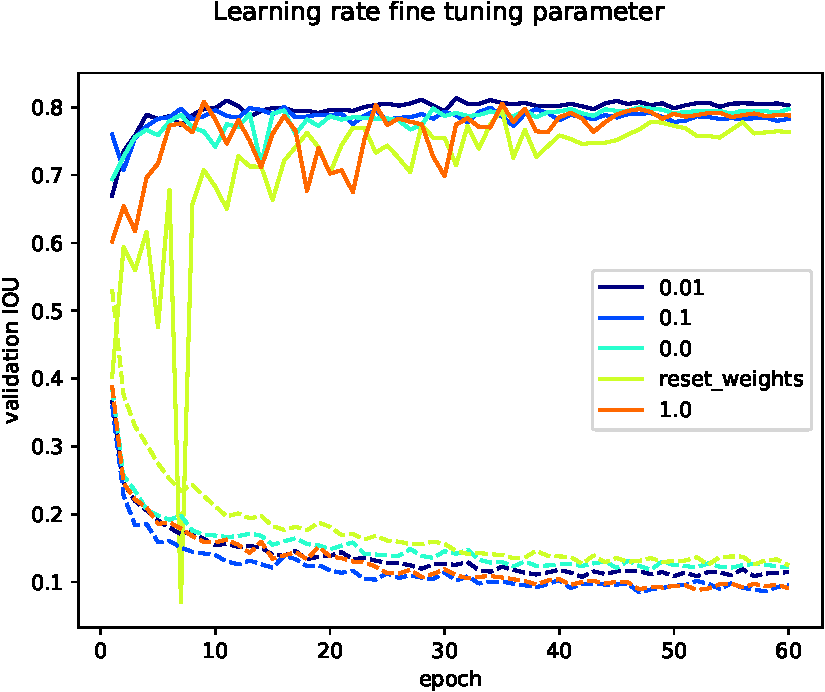
\includegraphics[width=0.9\linewidth]{bootstrap/fine_tuning.pdf}
  \caption{Influence of learning rate modifier for fine tuning}  
  \label{fig:fine}
\end{subfigure}%
\begin{subfigure}{.5\textwidth}
  \centering
  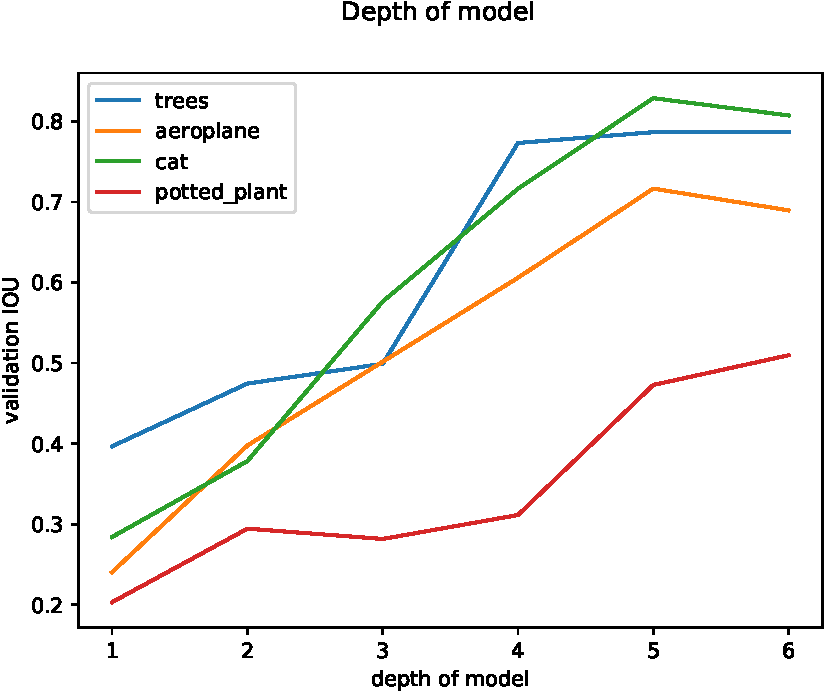
\includegraphics[width=0.9\linewidth]{bootstrap/depth.pdf}
  \caption{Depth of pre-trained model}  
  \label{fig:depth}
\end{subfigure}

\label{fig:training}
\end{figure*}




\subsection {Partial Annotation}


\begin{figure*}[!ht]
\centering
\begin{subfigure}[t]{.3\textwidth}
  \centering
  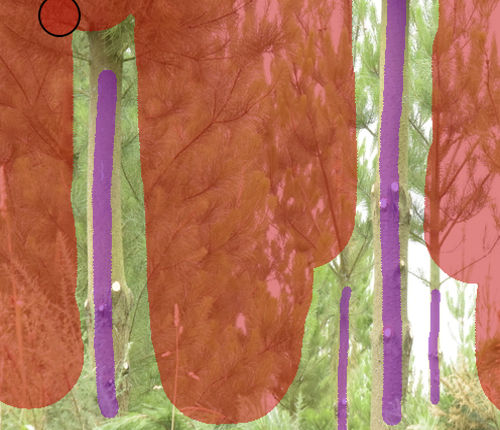
\includegraphics[width=0.6\linewidth]{bootstrap/loose.png}
  \caption{Partial annotation}
  \label{fig:loose_annot}
\end{subfigure}%
\begin{subfigure}[t]{.3\textwidth}
  \centering
  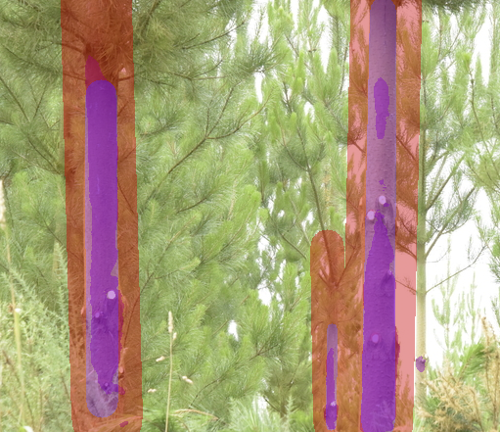
\includegraphics[width=0.6\linewidth]{bootstrap/loose_directed.png}
  \caption{Directed annotation}
  \label{fig:loose_dir}

\end{subfigure}%
\begin{subfigure}[t]{.3\textwidth}
  \centering
  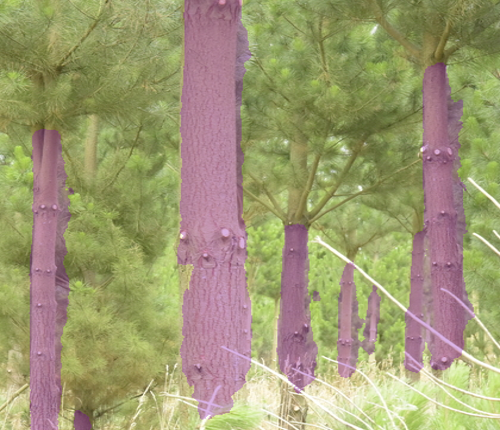
\includegraphics[width=0.6\linewidth]{bootstrap/loose_predictions.png}
  \caption{Predictions from partial annotation showing failure cases}
  \label{fig:loose_pred}
\end{subfigure}
  \caption{Loose annotation methods, red overlay refers to pixels labelled as background where transparent pixels are unlabelled}


\end{figure*}

\begin{figure}
\centering
\begin{subfigure}[t]{.15\textwidth}
  \centering
  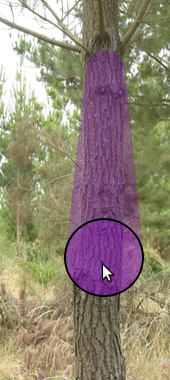
\includegraphics[width=0.7\linewidth]{bootstrap/line_tool.png}
  \caption{Line tool}
\end{subfigure}%
\begin{subfigure}[t]{.15\textwidth}
  \centering
  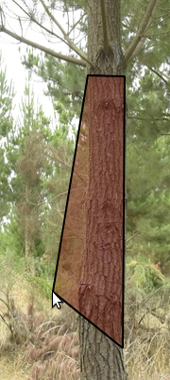
\includegraphics[width=0.7\linewidth]{bootstrap/polygon_tool.png}
  \caption{Polygon tool}
\end{subfigure}%
\begin{subfigure}[t]{.15\textwidth}
  \centering
  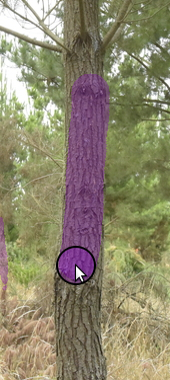
\includegraphics[width=0.7\linewidth]{bootstrap/paint_tool.png}
  \caption{Paint tool}
\end{subfigure}%

  \caption{Label paint tools used in annotation}
  \label{fig:tools}

\end{figure}



An alternative to densely annotating every pixel in an image is to selectively label some pixels while leaving many unlabelled - in the vein of the GrabCut algorithm. We examine this idea for a couple of reasons, firstly annotation all pixels is finicky or ambiguous (such as the small trees in the background), or secondly to optimise time spent on annotation only the most informative pixels (in the vein of active learning).

We firstly looked at partial annotation using paintbrush scribbles on the centre of trees and around the edges of the background. It can be seen that the model trained with partial annotation does not accurately find tree boundaries and has poor precision as a result as can be seen in Figure \ref{fig:loose_pred}. After identifying flaws in that process we compared directed annotation where we trained a model as we went in order to guide the annotation process.

For directed annotation we densely labelled the tree instances where there were mistakes, making sure to more accurately capture the boundaries. We were again annotating only a small number of easier instances where annotation was clear, unlike in the dense annotation case where many small and ambiguous instances are labelled.

Some statistics can be seen in table \ref{tab:loose_exp}, where we can see that both methods of partial annotation are less effective than dense annotation. The second method of directed annotation improves on the precision, but sacrifices recall. We can see that the extra supervision is indeed useful, and we lose useful supervision by not validating the model's correct output as well as fixing it's mistakes.


\begin{table}[!ht]
  \centering
    \caption{Statistics from re-annotation test set}

\noindent\resizebox{0.5\textwidth}{!}{%        
  \begin{tabular}{ l  l  l l l l l }
    Method & Positive pixels & Background pixels & Ignored pixels & Precision & Recall & IOU  \\
    \toprule
    Dense annotation	& 10.4\% & 89.6\% & 0\% & 87.8 & 87.3 & 77.8 \\
    Loose annotation	& 5.2\% & 67.4\% & 27.4\% & 82.3 & 83.3 & 70.7 \\
    Directed annotation & 7.2\% & 54.9\% & 38.0\% & 87.7 & 80.7 & 72.5 \\    
    \bottomrule
  \end{tabular}
}

\label{tab:loose_exp}
\end{table}






\subsection {Annotation interface experiment}



We performed an exercise in re-annotating the validation set using different tools. The results can be seen in table \ref{tab:annotation_exp}, where we used three approaches. The different tools used can be seen above in Figure \ref{fig:tools}.  The first being a duplication of the initial annotation using the line tool (the tool we initially used to label the dataset), the second being a polygon tool (more commonly used and general purpose than the line tool), and lastly we refined images produced by a trained model, fixing mistakes using the paint tool.

The model we used was a model trained on 30 images (densely labelled) from the loose annotation experiment above. We can see the method of refining model predictions is somewhat faster than the other two input methods, but due to the exercise being undertaken by a single user not significantly different ($ p > 0.01 $).

During the annotation we showed an image of the existing validation image and it's annotations side by side to the annotation software, this was necessary to ensure the same task was being performed. The smaller instances in each image were subject to the judgement of the annotator, and other images were extremely crowded or blurry leading to ambiguity in the annotation process. 



We can see from this exercise how tricky , given that two annotations using the same tool and using the other as a reference guide only managed a precision and recall of approximately $ 90\% $. All three methods were similar in this regard, but displayed different bias. The polygon tool for example (as used by the particular annotator) was more precise but less complete (lower recall), indicating that the user tended to cut within boundaries defined by the original labelling. 




\begin{table*}[!ht]
  \centering
    \caption{Statistics from annotating validation set in different ways. Precision, recall and IOU are a comparison with the original validation set. Note figures in brackets are the original statistics of the un-modified predictions from the model}

\noindent\resizebox{\textwidth}{!}{%    
  \begin{tabular}{ l  l  l  l  l  l  l  l }
    Method & Time/image & Edits/image & Pixels/image & Time/edit & Precision & Recall & IOU \\
    \toprule
    Polygon tool	& $79.3 \pm 35.0$  & $12.1 \pm 5.6$ & $52438 \pm 31900$   & $3.9 \pm 1.8$  & $0.94$ & $0.88$   & $0.84$ \\
    Line tool 		& $71  \pm 33.4$   & $12.2 \pm 5.6$ & $54781 \pm 33336$   & $2.1 \pm 1.4$ & $0.92$  & $0.90$  & $0.84$ \\
    Refine from model 	& $57.3 \pm 40.3$  & $10.8 \pm 6.1$ & $6561 \pm 7102$ 	  & $1.7 \pm 1.4$ & $0.92 (0.89)$   & $0.92 (0.85)$ & $0.85 (0.77)$ \\    
    \bottomrule
  \end{tabular}
}

\label{tab:annotation_exp}
\end{table*}


The confounding feature the annotation experiment was the need to look backward and forward between the two images in order to ensure the correct areas were annotated. In images with many instances, this became a difficult task and identifying small differences between the two became much more difficult. In future we may perform a more comprehensive user study, by providing an outline of the desired mask for the user to copy directly. This way the user does not spend any time comparing images and can focus only on the interaction (as a normal user of the annotation tool would).


\subsection{Practical considerations}

The need for more traditional validation for determining hyper--parameters, (for example training rate, model architecture) still need to be determined by validation as soon as enough examples have been obtained to be feasible. We performed some tuning of the hyper--parameters (for example the crop size, data augmentation parameters, learning rate) for the purposes of the experiments in this paper using the person category of the Pascal \gls{VOC} 2012 dataset, despite the fact that the tree dataset is significantly faster to train a similar set of hyper--parameters seems to have been suitable.


A practical consideration of having a process training a \gls{CNN} in the background, is that it uses a lot of (both CPU and GPU) resources. Running the trainer and the annotation tool together caused significant lag in the annotation tool which was not otherwise present and especially noticeable with a large batch size, the tool would lag in sync with each batch processed. The effect was that annotation became somewhat more time consuming. A simple solution to this would be to run processes on different machines with a web interface, for example.


\section{Future work}


In the future we intend to focus on more sophisticated methods of assisted annotation. We have already implemented some preliminary ideas, for example GrabCut with RGB-P such as proposed in \cite{Xu2016a}, utilising the model's predictions as another image channel.  Enhanced SuperPixels is another idea, however we found despite some improvement it suffered from many of the same problems as plain SuperPixels for small instances. 

In initially labelling our tree dataset we used drawing tools to create pixel masks, the problem with with pixel masks is twofold - firstly it is possible (and probable) for a model to make noisy predictions, secondly the pixel masks are not as easy to manipulate than the original primitives. For that reason we are interested in higher level prediction, where the model predicts the same high level primitives as the user first uses for input allowing for the full round trip. For example with our tree data set we draw trees using a line tool, then have the model predict those lines directly.


\section {Conclusion}

We proposed a bootstrapping method for rapid segmentation dataset creation, involving a feedback loop between human and model. The model trained on partial data is used to assist a human annotator, which then verifies the model's predictions and fixes any mistakes. We used this method to create a tree dataset for segmentation of Pinus Radiata trunks (for the purpose of finding trees requiring pruning). We then performed several experiments on this dataset, as well as the Pascal VOC in order to see how we might improve on this basic bootstrapping method. 

Through several experiments we determine that fine-tuning a pre-trained model is an effective way to obtain a workable model with very few input images, at least on our tree dataset. Partial annotation was explored and found to be less effective than a dense annotation. For this reason we think that it is more useful to create tools to assist the user to create a dense annotation, rather than making do with more approximate labelling. Alternatively in future we may focus on methods allowing for a round trip using high level primitives.





\chapter{The Role of Focus in Object Instance Recognition}



% As a general rule, do not put math, special symbols or citations
% in the abstract

We present a study on the effects of focus on object instance recognition (identifying instances of the same object or very similar object, for example a particular product) using Convolutional Neural Networks. The field of object detection is seen as an harder task than that of recognition, as the object must be localised as well as classified. In the field of face recognition, alignment is seen as a crucial step for the purpose of recognition - it is our hypothesis that focus and alignment is similarly important for object instance recognition. 

We perform some experiments to verify the effects of localisation, using datasets with bounding box annotations. We found that CNN classification on images cropped to bounding box regions is much more accurate than classification of whole images. Both magnification and centring of the object in question seem to also have a strong effect, and including context in the classification is only useful if it does not come at the expense of minifying the object to be classified.
 
We conclude in order to produce a quality instance recognition using \gls{CNN}s for classification, it would be a large advantage to first localise and then focus on the region of interest. Future research will focus on how this localisation can be performed, for example using a model to first estimate a bounding box and rotation using regression, or using Spatial Transformer Networks which enable learning a joint classification and focus method.




\section{Introduction}

Object detection is described typically as a harder problem than object recognition only, for the reason that it requires not only classifying which object is present, also establishing where each object is located. We look at this from another angle, if we can first focus on the location each object is located - can we do a much better job of identifying which object is present? 

Convolutional Neural networks (\gls{CNN}s) \cite{LeCun1998} have become the tool of choice for image classification problems in recent years. Despite having been invented many years earlier it was the advent of GPUs enabling larger datasets and larger networks which triggered adoption, initially coming to prominence in \cite {Krizhevsky2012}.  We experiment with how focus influences the performance of a CNN model for the purpose of instance recognition. Our interest is in instance recognition, we can see that these ideas are not unique to instance recognition but for object recognition and classification with \gls{CNN}s in general.

\gls{CNN}s are said \cite{Krizhevsky2012}, to having properties which make them invariant to translation, and naturally learn redundancy to scale and rotation present in the training data. Is it necessary then, that \gls{CNN}s, must be focused and aligned on the exact area of interest? The role of focus and alignment can be seen most clearly in face recognition, where faces are aligned very precisely. Face recognition almost ubiquitously uses alignment as a pre-processing step, before passing images on to a model for recognition purposes even when the model is a deep CNN \cite{Taigman2014}.

It seems intuitive that focusing on the relevant part of an image should produce a better outcome, however we're also aware that the context of an object is said to be important in recognition \cite{Oliva2007}. For example the background of water and sky gives a strong clue that the object is more likely to be a boat than a car. A cluttered background is seen as a problem in object recognition and detection, and it was noticed in an effort to compare image patches, that prioritizing pixels in the centre of a patch \cite{Zagoruyko2015} increased performance. In this light -- it is unclear if including context in image classification is always advantageous. 

We look at this in the context of object instance recognition with two datasets where objects have been localised with bounding boxes. We use two instance recognition datasets the Washington RGB-D dataset \cite{Lai2011} of object turntable sequences, and the INSTRE dataset \cite{Wang2015} containing photographs of objects captured by hand. In the case of the INSTRE dataset, most (but not all) objects are captured with backgrounds where context is not very predictive - for example a toy captured with a grassy background. The RGB-D dataset is captured in a controlled environment with a white turntable in the background in all images.

\gls{CNN}s are frequently used to learn alignment, for example bounding box regression as is common in object detection \cite{Sermanet2013}. In face recognition facial features are commonly detected and used to align the face very closely with other face images, which is also typically performed using a CNN. For the generic task of object instance recognition we don't have the luxury of obvious landmarks for alignment, as they vary largely depending on the type of object, but we can consider more general alignment such as estimating bounding box(es) or using regression to estimate rotation as in \cite {Fischer2015}. 

Spatial transformers \cite{Jaderberg2015} are another option and enable a joint learning of a classifier and attention method (affine transformation) for \gls{CNN}s, with evidence they  house numbers in natural images \cite{Netzer2011} and bird species recognition \cite{Wah2011} In future we will evaluate these alignment methods for the purpose of object recognition as well as consider methods of capturing object images with bounds and orientation, if identifying the correct focus is more difficult than recognition there is little point.


\section{Method}

We use the same training method, and optimisation method throughout, except where mentioned the parameters are as described in this section. 

\subsection {Learning}

We use standard \gls{SGD} with momentum set to $ 0.9 $. We set the learning rate to $ 10^{-2} $ and interpolate this rate across each epoch to a minimum of $ 10^{-4} $. We interpolate the learning rate using \gls{SGDR}  \cite{Loshchilov2016}, however we reduce the learning rate at each mini-batch instead each epoch. We set our epochs to be relatively large accordingly, and restart SGD at the higher learning rate at the beginning of each epoch. 

Each training cycle was performed with epoch sizes of 65536, and 10 epochs were trained in all cases, after which the loss function plateaued. We use a mini--batch size of 64, an image size of $64\times64$ (though this is varied for some experiments). We select images from each class randomly with uniform probability, as well as images from within each class with uniform probability.

\subsection {Network}

We use the same architecture CNN in each case, varying slightly for experiment two where we increase the pixel size of the input image (see below for details). We use a simple AlexNet \cite {Krizhevsky2012} style model, details are given in table~\ref{fig:focus_network}. Other network architectures, such as the popular ResNet \cite{He2015} style were evaluated, and perform very similarly at the tasks presented here, at the expense of taking longer to train.

Each convolution operation is padded, in order that inputs and outputs dimension match (e.g $ 7\times7 $ convolutions have inputs zero padded by 3 pixel, and $3\times3$ convolutions have inputs zero padded by 1 pixel). It can be seen that each layer (ConvLayer) halves the input resolution after convolution, using max-pooling. For a non linearity we use the \gls{PRELU}. Batch Normalisation is used directly before all convolution layers and uses a running sum with momentum = 0.9.

Our classification method is the standard SoftMax method with the usual cross entropy loss function. Before the final linear layer we use a single dropout layer $ p = 0.5 $, which we have found prevents over-fitting even though it is said to be unnecessary to use both Batch normalisation and dropout.  We use the Torch7 \cite{Collobert2011a} neural network library to implement this network and perform all experiments. 

\begin{table}[h]
  \centering
    \caption{Neural network structure }
\begin{tabular}{ l } 

\toprule

 ConvLayer(n) = PRelU $\rightarrow$ Batch Normalisation \\ 
 $\rightarrow$  Convolution $(3\times3, n \rightarrow n * 1.5)$ $\rightarrow$  Max Pooling $(2\times2)$ \\
\\
 LinearLayer(m, n)  = PRelU $\rightarrow$ Batch Normalisation \\  $\rightarrow$  Linear $(m \rightarrow n)$ \\
\toprule
  Network = Batch Normalisation $\rightarrow$
 Convolution $(7\times7, 3 \rightarrow 32)$ \\
 $\rightarrow$ Max Pooling $(2\times2)$   \\

  $\rightarrow$ ConvLayer (32) $\rightarrow$  ConvLayer (48) $\rightarrow$ ConvLayer (72) $\rightarrow$ ConvLayer (96)   \\
  
  
  $\rightarrow$ Flatten $(2\times2\times144 \rightarrow 576)$ $\rightarrow$ LinearLayer (576, 256) \\
  
  $\rightarrow$ Dropout(0.5) $\rightarrow$ LinearLayer (256, $\vert classes \vert$ )  $\rightarrow$  SoftMax($\vert classes \vert$) \\
  
    
       
\toprule
\end{tabular}

\label{fig:focus_network}
\end{table}




\subsection {Image Preparation and Pre-processing}


\begin{figure*}[t]
    \caption{Examples of data augmentation }
\centering
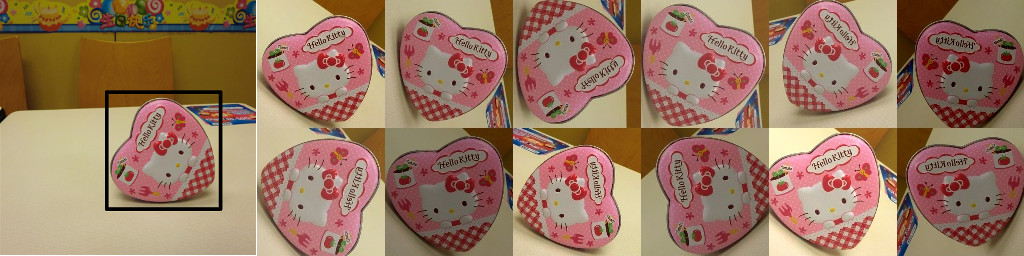
\includegraphics[width=1.0\textwidth]{focus/image_variations.jpg}
\label{fig:focus_variations}
\end{figure*}


In cropping an image to it's object's bounding box, we use a uniform scaling -- in order to ensure the entire object fits within this bounding box we fit a square around the bounding box in the cases where the bounding box is not square (we use square images as inputs to neural networks in this work).

We used data augmentation heavily to regularise the training in the form of random image transformations. Training images are randomly transformed using a set of parameters sampled from a normal distribution and shown in table \ref{fig:focus_jitter}.  We use translations, rotation about the centre, scales (uniform and non uniform), brightness and contrast adjustments. Testing images are re-sized and cropped in the same way (described below), but with no random transformations. An example of training data is given in figure~\ref{fig:focus_variations}.

\begin{table}[h]
  \centering
    \caption{Ranges of parameters used for image distortion }
    
  \begin{tabular}{ l  l }
    Parameter & Mean $ \pm $ Standard deviation \\
    \toprule
    scale (uniform) & $ 1 \pm 0.2 $  \\ 
    non uniform scale  & $ 1 \pm 0.2 $  \\ 
    rotation (degrees) & $ \pm 90 $ \\ 
    translation(x, y) (\% image size) & $ \pm 5 $ \\ 
    brightness (additive) & $ \pm 20 $ \\ 
    contrast (multiplicative) & $ 1 \pm 0.2 $ \\ 
    \bottomrule
  \end{tabular}
\label{fig:focus_jitter}
\end{table}


An affine transformation matrix $ (2 \times 3) $ is computed, firstly scaling the image to fit the bounding box region to match the network's input size, applying a set of random transformations as above, then cropping a rectangular region around the origin of the transformed image. We use OpenCV's warpAffine function to perform this as a single step, avoiding artifacts from multiple image transformations (and also to avoid having to compute intermediate images with associated clipping issues).

\subsection{Datasets}

The RGB-D \cite{Lai2011} dataset which contains turntable images with a fixed camera at 30 degrees, 45 degrees and 60 degrees of elevation. For evaluating instance recognition the 30 and 60 degree images are used for training, and the 45 degree images used for testing. Bounding boxes are provided for each image (generated using depth information). The RGB-D dataset contains approximately 500 images (varying a little) for each instance, with 300 different object instances. We make no use of the depth images provided in the dataset.

The INSTRE \cite{Wang2015} aims to be a more diverse, better balanced dataset with cluttered backgrounds than existing object instance recognition datasets. It improves on the RGB-D dataset in that the range of views are much more varied, the types of object have more variety, the backgrounds have variety (hand taken photos) rather than the turntable background. Bounding boxes are again provided. No standard test set is provided for the INSTRE dataset, so we take images of each object for testing, and use the remaining images for training at a ratio of $1:3$. The INSTRE dataset contains 200 classes of object, each with 100 images which have either been hand captured or picked. 

The INSTRE dataset contains unique challenges. A number of the objects are a little abstract, and include things like logos (e.g. one of the categories is KFC, which includes pictures of the building prominently showing the logo, as well as napkins containing the logo and pencil drawings). An example hard case is shown in figure~\ref{fig:focus_adidas}. Many categories feature objects rotated in numerous ways, with both landscape and portrait images, as well as many photos taken on angles with no alignment at all.

\section {Experiments}


\subsection {Experiment 1}

Our first experiment compares the effect of focusing on the bounding box on classification accuracy. If we had an oracle which could give us a bounding box estimate (or another model which could accurately give a bounding box estimate) - how much better is the network performance on cropped versus baseline (uncropped) images? We apply this cropping equally on test and training images.

For the RGB-D dataset, which for many of the objects only occupy a tiny space of the full image, we crop the inner centre 40 percent of the image for the uncropped baseline. Otherwise, after scaling the original image to $ 64 \times 64 $ the smaller objects occupy only a few pixels, with the turntable and background being vastly bigger in scale. In order to see if the magnification from cropping to the bounding box was having an effect, we also ran the baseline at a higher resolution - but noticed little change in performance.


\begin{table}[h]
  \centering
    \caption{Cropped vs. uncropped images }
    
  \begin{tabular}{ l l l }
    
    Dataset & Image preparation & test set accuracy \\
    \toprule
    
    INSTRE & baseline &  65.3 \\
    INSTRE & bounds cropped & 89.0 \\
    
    RGB-D & centre cropped & 58.1 \\
    RGB-D & bounds cropped & 81.6 \\
    
    \bottomrule
  \end{tabular}
\label{fig:focus_crop}
\end{table}

The RGB-D results suggest over-fitting, with the training accuracy reaching almost 100 percent, yet generalising badly to the test set. The RGB-D images present a problem in that the test set (those images captured at 60 degrees elevation), are from a slightly different distribution from the training (they're captured at a constant level of elevation). Each image is also reasonably redundant due to being part of a video sequence. A potential solution to this is using a higher level of randomised non uniform scaling when training. The INSTRE images on the other hand have no systematic difference between training and test images and also cover a much greater intra object variety and do not show the same kind of over-fitting.

It is clear that focusing on the bounding box has a large impact on the performance of the classification, with both RGB-D and INSTRE classification improved when trained and tested on images cropped to the bounding box. Given this is the case, we seek to discover exactly why. Which property which enables effective classification using this kind of CNN model? Is it the magnification of the object after cropping an image to the bounding box or removing the distracting background? (It is clear the object is much larger in pixels after the resulting image is scaled to match the CNN input size). Or is it the centring of the object, suggesting the translation invariance of the CNN is not as general as is widely assumed?


\subsection {Experiment 2}

\begin{figure*}[t]
    \caption{Examples of cropping for context}
\centering
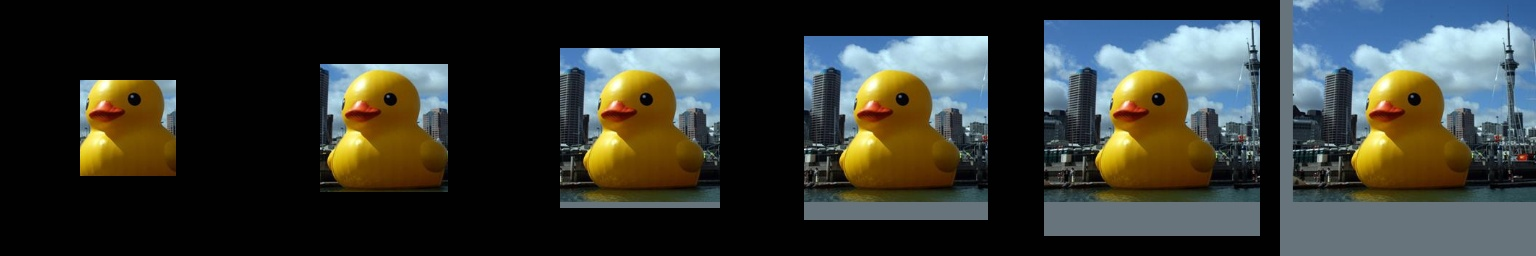
\includegraphics[width=1.0\textwidth]{focus/enlarge.jpg}
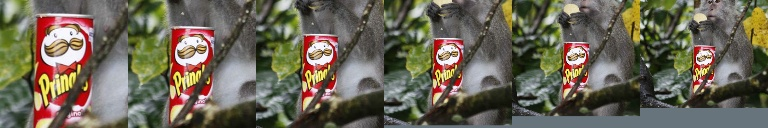
\includegraphics[width=1.0\textwidth]{focus/shrink.jpg}
\label{fig:focus_context}
\end{figure*}




\begin{figure}[h]
    \caption{Context in image classification vs. test set accuracy}
\centering
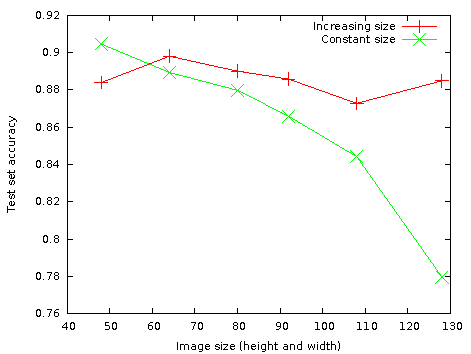
\includegraphics{focus/graph.pdf}
\label{fig:focus_exp2}
\end{figure}

For our second experiment we explore how including context changes the performance. We do this in two ways, firstly by fixing the pixel size of our object and including more context by using a larger input image to the model, secondly by fixing the size of the input to the network and including the same context, where the object is scaled down to accommodate.

In the first case we scale the object bounding box to $ 64 \times 64 $ and set this as the base scale, each larger size includes proportionally more context where the object remains a constant size in pixels. In the second case we use a fixed image size of $ 64 \times 64 $, using the same image context for each size as the first case, causing the object to be relatively scaled smaller.

The architecture of the network is mostly unmodified (each image output within the hidden convolutional layers in the network is of a larger dimension). The number of parameters is constant for the convolutional layers, but the first fully connected layer contains a larger number of inputs to cope with the extra outputs from the convolutional part. The differences can be seen in table~\ref{fig:focus_sizes}.


\begin{table}[h]
  \centering
    \caption{Example output sizes for input dimensions }
\begin{tabular}{ l l l } 
 
 \toprule
 Input image size & Convolution outputs & Flattened size \\
 \toprule
 
 $ 48 \times 48 \times 3 \rightarrow $ & $ 1\times1\times144 \rightarrow $ & 144 \\
 $ 64 \times 64 \times 3 \rightarrow $ & $ 2\times2\times144 \rightarrow $ & 576 \\
 $ 108 \times 108 \times 3 \rightarrow $ & $ 3\times3\times144 \rightarrow $ & 1296 \\
 $ 128 \times 128 \times 3 \rightarrow $ & $ 4\times4\times144 \rightarrow $ & 2304 \\
 
\end{tabular}
\label{fig:focus_sizes}
\end{table}

We can see from the data shown in figure~\ref{fig:focus_exp2} that performance is relatively constant where the scale of the object is fixed. Adding context neither gives a performance boost nor hinders recognition (only takes longer to train). Where context is added at the expense of the object scale we can see that at the higher levels the test accuracy drops.


\subsection {Experiment 3}

Given the results from experiment~2, it seems that reducing the scale of the object (in pixel size) causes a degradation of the performance. Experiment~1 shows that the unmodified INSTRE images are still much more difficult to classify for a CNN. Experiment 2 normalises scales between objects (for example.e. the statue of liberty becomes the same size in terms of image pixels as a can of cola). For experiment 3 we use the bounding box to centre the object, but leave the scale unmodified.


\begin{table}[h]
  \centering
    \caption{Effect of input size and centring}
    
  \begin{tabular}{ l l l l }
    
    Dataset & Input size & Test set accuracy \\
    \toprule
    
    INSTRE &  $ 64 \times 64 $ & 65.3 \\
    INSTRE &  $ 128 \times 128 $  & 71.7 \\
    INSTRE &  $ 192 \times 192 $  & 76.0 \\
    
    \toprule
    INSTRE (centred) &  $ 64 \times 64 $ & 71.6 \\
    INSTRE (centred) &  $ 128 \times 128 $  & 80.6 \\
    INSTRE (centred) &  $ 192 \times 192 $  & 84.2 \\
    
    
    
    \bottomrule
  \end{tabular}
\label{fig:focus_input_size}
\end{table}



We can see from this experiment that both increasing magnification, as well as centring the object both give significant accuracy boosts, not to the same level as cropping to the bounding box, but close. Perhaps even larger magnification would be fruitful. 

The fact that centring the object makes such a difference is surprising, given the translation invariance of the CNN architecture, however it is not clear exactly how much a CNN is translation invariant (even though we can see that the filters used in a convolution step are clearly translation invariant - it is not obvious that the network as a whole possesses such properties). A recent study attempting to quantify this translation invariance \cite{EricKauderer-Abrams2016} suggests the architecture, and data augmentation are both important here. 


\subsection {Failure cases - discussion}


\begin{figure*}[t]
    \caption{Example of one hard case in the INSTRE dataset}
\centering
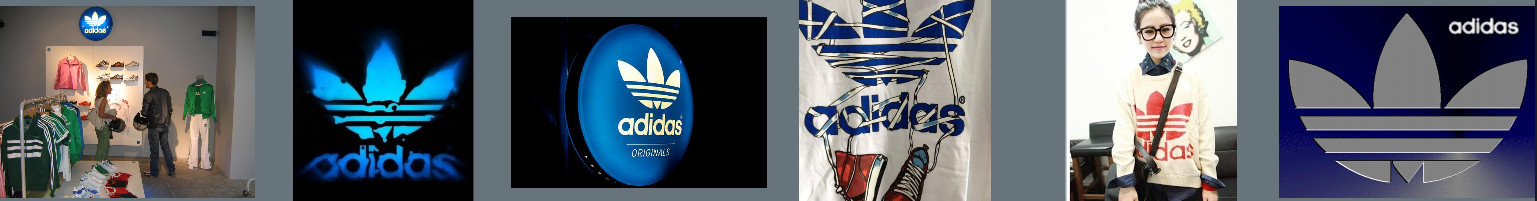
\includegraphics[width=1.0\textwidth]{focus/adidas.jpeg}
\label{fig:focus_adidas}
\end{figure*}



\begin{table}[h]
  \centering
    \caption{Worst categories in testing }
  \begin{tabular}{ l l }
  wangzai & 46.6 \\
  einstein bros & 46.6\\
  Manneken Pis & 45.4\\
  mastermind JAPAN & 45.1\\
  clapperboard & 43.2\\
  Che Guevara & 38.2\\
  coca cola & 33.3\\
  Paul Frank Julius & 32.4\\
  Kung Fu Panda & 24.0\\
  Adidas Originals & 17.2\\
    \bottomrule
  \end{tabular}
\label{fig:focus_failure}
\end{table}

It can be seen in figure~\ref{fig:focus_failure}, that many of the worst performing object classes were those which are somewhat abstract, for example logos which were stylistically the same logo but appeared visually quite different with different colours, materials and occurring in very different contexts. An example is shown in figure~\ref{fig:focus_adidas} for the ``Adidas Originals'' object.



\section{Conclusion}

We found that CNN classification on the cropped bounding box regions is much more accurate than classification of whole images. Both magnification and centring of the object in question seem to have a strong effect (which is somewhat surprising, given the translational invariance properties of CNN models). On the experiments we performed, including context in the input images was only useful if it does not come at the expense of minifying the object (reducing it's pixel size) to be classified.

We conclude in order to perform quality instance recognition using \gls{CNN}s for classification, it would be a strong advantage to first localise the region of interest, and then focus on the region of interest.  In future we will both further investigate why we see the results above, and at the same time peruse how focus methods can be used to improve instance recognition. Understanding the failure modes in unfocused image classification is also of interest, understanding in more depth our observations. For the INSTRE data set, the more abstract categories were among those which failed to generalise well, and RGB-D dataset simply over-fit badly.

We will explore bounding box regression as is used in many object detection methods, as well as rotation regression for the purposes of aligning input images to a canonical orientation. One difficulty with using regression is the requirement that your training data requires annotation, making it's use in practice more expensive to obtain. Alternatives include using using external data, and using methods of semi-automated segmentation (for example using a green screen). Alternatively, the use of Spatial Transformer networks is interesting -- which require no such annotation, which jointly learn the focus method with the classifier.





\documentclass{llncs}
\usepackage{epsf}
\usepackage[pdftex]{graphicx}
\usepackage[acronym]{glossaries}
\usepackage{booktabs}
\usepackage{gnuplot-lua-tikz}
\usepackage{tikz}
\usepackage{amsmath}

\usepackage{enumitem}
\setlist{parsep=0pt,listparindent=\parindent}

\input{ps-fig.tex}

\renewcommand{\tabcolsep}{0.2cm}

\begin{document}

\title{Object~Recognition~by
      Stochastic~Metric~Learning}


\author{Oliver Batchelor, Richard Green}
\institute{Department of Computer Science\\
	   University of Canterbury\\
	   Christchurch, New Zealand\\
	   oliver.batchelor@pg.canterbury.ac.nz, richard.green@canterbury.ac.nz}          
           
\maketitle

\makeglossaries


\newacronym{CNN}{CNN}{Convolutional Neural Netowork}
\newacronym{MCDNN}{MCDNN}{Multi Column Deep Neural Network}

\newacronym{SIFT}{SIFT}{Scale Invariant Feature Transform}
\newacronym{SURF}{SURF}{Speeded Up Robust Features}

\newacronym{ALOI}{ALOI}{Amsterdam Library of Images}
\newacronym{MSR}{MSR}{Microsoft Research}

\newacronym{BOW}{BoW}{Bag of Words}
\newacronym{BOVW}{BoVW}{Bag of Visual Words}

\newacronym{ANN}{ANN}{Approximate Nearest Neighbor}
\newacronym{SGD}{SGD}{Stochastic Gradient Descent}
\newacronym{ASGD}{ASGD}{Asynchronous Stochastic Gradient Descent}
\newacronym{LOO}{LOO}{Leave One Out}

\newacronym{NCA}{NCA}{Neighborhood Components Analysis}
\newacronym{MEGM}{MEGM}{Mean square Error's Gradient Minimization}

\newacronym{KNN}{kNN}{k-Nearest Neighbor}

\newacronym{MSE}{MSE}{Mean Squared Error}
\newacronym{LMNN}{LMNN}{Large Margin Nearest Neighbor}
\newacronym{SVM}{SVM}{Support Vector Machine}

\newacronym{PCA}{PCA}{Principle Components Analysis}
\newacronym{DRLIM}{DrLIM}{Dimensionality Reduction by Learning an Invariant Mapping}
 
\newacronym{GPU}{GPU}{Graphics Processing Unit}

\begin{abstract}

Descriptors extracted from deep neural networks have been shown to be very discriminative,
for example networks such as those trained on the large, very general ImageNet dataset have been used to extract descriptors robust for a variety of image classification tasks. Such retrieval systems utilize feature locality, for example Approximate Nearest Neighbour. Our goal is to use such descriptors as part of a large scale object instance recognition and retrieval system. We propose using deep nonlinear metric learning on Convolutional Neural Networks to learn features with good locality. In particular we worked with two related methods, \gls{NCA} and the related \gls{MEGM}.

We utilize a nonlinear form of \gls{MEGM} as an alternative to \gls{NCA} and propose some stochastic sampling methods to apply these (normally batch) methods to larger datasets with minibatch \gls{SGD}. On a larger scale we found the methods difficult to train, failing to converge or generalizing very badly depending on training method or parameters. This led us to go back to a smaller dataset and examine the factors which lead to good generalization with this form of training.
  
We found on a small subset of the RGB-D dataset, surprisingly stochastic sampling methods generalized much better with small batch sizes, which acted as a form of regularization. When trained with larger batches, or as a full batch, the dataset was overfit. Given the correct parameters, descriptors extracted performed well at the Nearest Neighbour task and exceeded the performance of those extracted by applying standard supervised training.


\end{abstract}

\section{Introduction}

Deep convolutional neural networks in combination with modern GPUs and large image datasets have shown strong performance on image classification tasks \cite {Krizhevsky2012}, and has been applied to related problems such as object detection \cite{Sermanet2013}, image segmentation \cite{Masci2013} and image retrieval \cite{Razavian2014}.

\subsection {Descriptors from Deep Neural Networks}

Using descriptors derived from the hidden layers of a neural networks trained using supervised learning, for the purpose of other learning tasks is a relatively new idea. These descriptors have been shown to be robust even for quite unrelated tasks \cite{Donahue2014,Razavian2014}. The ImageNet dataset \cite{Socher2009} is a popular source for pretraining, and pre-trained models exist such as the OverFeat network \cite{Sermanet2013} or the DeCAF feature extractor \cite{Donahue2014}). 

A standard technique in training a \gls{CNN} is to augment the dataset by applying transformations, more data typically gives better generalization. In \cite{Dosovitskiy2013}, a \gls{CNN} was trained on single images which were warped in many different ways. Features obtained from the network were then used in popular classification benchmarks achieving good results. For many years local image descriptors such as \gls{SIFT} \cite{Lowe2004} have been used for matching and indexing images, a recent comparison \cite{Fischer2014} (though perhaps not a fair one) showed that using a \gls{CNN} for matching tasks performed better than \gls{SIFT} by a margin similar to the improvement given by \gls{SIFT} to raw pixel data.


The final layer of a standard deep neural network as used in supervised classification consists of a set of linear classifiers, as such those descriptors are suitable for classification using other linear classifiers such as SVMs. Nearest Neighbor suffers from high dimensionality and noisy or irrelevant dimensions, as such the descriptors produced by a CNN may not be suitable for comparison by distance. For that reason we have looked towards metric learning to directly optimise the descriptors for the purpose of Nearest Neighbor classification. 


\subsection {Deep Metric Learning}


Metric learning has often been used for object recognition and image classification \cite{Hadsell2006,Min2009} (and many others), and especially face recognition, for example \cite{Kostinger2012}. Although most efforts often have focued on mahalanobis distance metric learning (a form of distance metric learning linear transformation), deep metric learning has had some attention \cite {Salakhutdinov2007a,Min2009,Weston2009,Min2010}. At the expense of much larger computation cost, deep metric learning has been shown to perform much better than its linear counterparts. We use gradients from metric learning to drive \gls{SGD} on a deep \gls{CNN}. 

\subsection {Training}

Metric learning comes with its own set of challenges, it has often been formulated as batch training method because each example potentially interacts with every other example. In practice descriptors from examples far apart don't interact with each other at all, so approximations can be made as we discuss later. This runs into issues relating to high dimensional spaces, namely the ``curse of dimensionality''. In high dimensional spaces, such as those we deal with in this paper, if the points (descriptors) were uniformly spaced then on average the number of neighbours increases with dimension. 

The interaction between points decays with distance (for example exponentially with \gls{NCA}). We can use approximations around the local neighbourhood of examples which can be used to create an \gls{SGD} training proceedure. Using an approximation to the nearest $ k $ neighbours is a popular approach, seen in \cite{Mensink2012,Zaidi2011} (of many). Clustering (amongst other sampling methods) is discussed in  \cite{Oneat2011} such as Farthest Point or Random Projection clustering, the downside of such clustering is that it is hard to control the size of a batch. 

Many training methods focus on interaction between pairs of (similar/dissimilar) examples or triples (example, more similar, less similar), for example DrLIM \cite{Hadsell2006} where a spring analogy is used to create an attraction between similar pairs and a repulsion between dissimilar pairs, the advantage with this kind method is that it can be used without explicit class labels, but just a similar/dissimilar annotation.

\section {Deep Metric Learning}

A deep neural network (in our case a \gls{CNN}) is used to to create an embedding into a lower dimensional space, creating descriptors which can be compared with their euclidean distance (and classified with nearest neighbour) where the euclidean distance of the raw pixels is both expensive and not a good measure of the distance of the semantic similarity of image content. 

We examine non linear versions of two methods \gls{NCA} \cite{Goldberger2004}, the closely related, but less well known \gls{MEGM} \cite {Zaidi2011}. \gls{NCA} optimizes a continuous version of the \gls{LOO} performance, it uses a softmax over weights which decay exponentially with distance. The \gls{NCA} score can be interpreted as the probability that a descriptor will pick another descriptor of the correct class as its nearest neighbour. 

The probability, $ p_{ij} $, of one descriptor selecting another descriptor, as its neighbour is defined as a softmax function over weights $W_ij$. The indexes $ i $ and $ j $ refer to input examples $x_i$ and $x_j$, and corresponding vector valued output of a \gls{CNN} $f(x_i)$ and $f(x_j)$ which are the descriptor vectors.

\begin{equation}
\label{eq:nca_prob_pair}
p_{ij} =  \frac {W_{ij}} {\sum_{k \neq i}{W_{ik}}}g
\end{equation}

Then the total probability, $ p_i $, of a point selecting any neighbour with another with its \emph{correct} class is defined as the sum of those neighbour probabilities $p_{ij}$ which have the same class:

\begin{equation}
\label{eq:nca_prob}
p_{i} =  \sum_{j:c_j = c_i}{p_{ij}}
\end{equation}

Where $ C_i $ is the class label of example $ i $. We use a gaussian kernel for the weighting as \cite{Zaidi2011} do. 

\begin{equation}
 \label{eq:gaussian_kernel}
W_{ij} = exp(\frac{-\lVert f(x_i) - f(x_j) \rVert^2_2 }{2\sigma^2}), \space W_{ii} = 0
\end{equation}


Then the function to be maximized, is the total sum of the probabilities of all descriptors being correctly classified.

\begin{equation}
\label{eq:nca_loss}
\mathcal{E}_{nca} =  \sum_i {p_i}
\end{equation}

Where \gls{NCA} optimises directly on the probability $ p_{i} $ above, \gls{MEGM} instead computes for each class $ \hat{y_{ti}} $ as a prediction that a descriptor will take class $ t $, where the only difference is that $ c_j = t $ as opposed to $ c_j = c_i $:

\begin{equation}
\label{eq:megm_pred}
\hat{y_{ti}} = \frac{\sum_{j:c_j = t}W_{ij}}{\sum_{k \neq i}{W_{ik}}}
\end{equation}

The prediction $ \hat{y_{ti}} $ can then be compared with $ y_{ti} $ (1 where $ t = c_i $, 0 otherwise), it then minimizes the \gls{MSE} between prediction and true class label:

\begin{equation}
\label{eq:megm_loss}
\mathcal{E}_{megm} =  \sum_i\sum_t{(y_{ti} - \hat{y_{ti}})^2}
\end{equation}

Intuitively \gls{MEGM} can be seen to penalize the case where two classes compete for the same region more so than when one class competes against examples of many different classes, where as \gls{NCA} would treat the two cases approximately equally. These loss functions can be used to drive gradient descent on a \gls{CNN} by standard backpropogation. The derivative for \gls{MEGM} is shown in the appendix, section~\ref{sec:appendix}.

We compute the gradient over the outputs of each minibatch and apply backpropogation as usual to find the derivative with respect to the weights of the network. It can be noted that the output, and derivative for \gls{MEGM} is more expensive to compute because of the additional per class summation, so it would not be suitable with an extremely large number of classes. In practice a large number of the terms can be factored out and precomputed, as well as computing the difference summations in terms of matrix multiplication.

Note the parameter $ \sigma $ was not in the original NCA, and is initialized to the average distance to the nearest neighbours of the initial descriptor output before training. We use it to prevent the weights initializing to zero when the distance between descriptors is large.


Where $\alpha $ controls the tradeoff. When $ \alpha \mathcal{E}_{mse} > \mathcal{E}_{nca} $ the descriptors all collapse into the same point.


\section{SGD for metric learning}

Our main proposal is in using minibatch \gls{SGD}, and applying it to metric learning methods which have been designed as batch learning methods. Metric learning as shown above as a batch method, scales at $ O(n^2) $ for $ n $ examples. Given that we wish to apply these approaches to large datasets containing hundreds of thousands or millions of images we are forced to consider approximations. The typical method for training a \gls{CNN} on large numbers of images is using \gls{SGD}, because it is fast, simple and scales to handle large datasets easily. 

The most obvious approximation is to just truncate the influence to the nearest $ k $ neighbours as the weight exponentially decays with the square distance. We hypothesised this would lead to the best approximation, however there are many ways of truncating the neighbourhoods. This lends itself to clustering methods and is more complicated than the alternative, which is to sample batches randomly, but use a large enough batch to include several examples of each class.

We propose the following approaches for sampling batches for \gls{SGD}:

\begin{enumerate}
\item {\bf Random shuffled batches}
 Randomly shuffle the dataset and divide up into batches of a fixed size, exactly how batches would normally be selected for supervised learning. Each batch contains (almost certainly) different numbers of examples from each class.
 \item {\bf Stratified random batches} 
 Pick batches by selecting a number of examples from each class, to ensure the same number of examples of each class are represented in each batch.   

 \item {\bf K-neighbourhoods around random points}
 Before each training epoch, run the model forward through the training set to obtain descriptors for each example. Select N examples at random and pick the batch as the batch sized neighbourhood (in descriptor space) of each selected example.
\end {enumerate}


\subsection {Issues of Scale}

The parameter $ \sigma $ is largely optional in theory, as the scale can be factored into the final fully connected weight matrix (or previous layers).  We make use of $ \sigma $ for the purposes of numerical stability upon initialization, during training the density of points adjusts itself to fit this parameter. It can also be observed that for different values of $ \sigma $ that the distance between descriptors adjust themselves to fit the new parameter over a few iterations of training.


\subsection {Adding Mean Square Error}

We experimented with adding the square distance between members of the same class as a means of adding some bias to the loss functions after suspecting that metric learning methods decribed above were overfitting, to force the output distribution to be more simple. 

\begin{equation}
\label{eqn:mse}
\mathcal{E}_{mse} = \sum_i{ \sum_{j:j_c = i_c}  \frac {{\lVert f(x_i) - f(x_j) \rVert^2_2}} {\sigma^2} }
\end{equation}

\begin{equation}
\label{eqn:mse_total}
\mathcal{E}_{total} =  \mathcal{E}_{nca} + \alpha \mathcal{E}_{mse}
\end{equation}


\subsection {kNN implementation}

We use a brute force \gls{KNN} algorithm running on CUDA \cite{Garcia2008}, computing the distance matrix using matrix multiplication followed by using an insertion sort to select the $ k $ neighbours of lowest distance. This approach is not scaleable to large datasets, and smarter clustering algorithms will eventually need to be used, however the time for evaluating \gls{KNN} on the datasets we experimented with are still dominated by the cost of computing descriptors from examples. 


\section {CNN architecture}


\begin{figure}[ht]
\centering
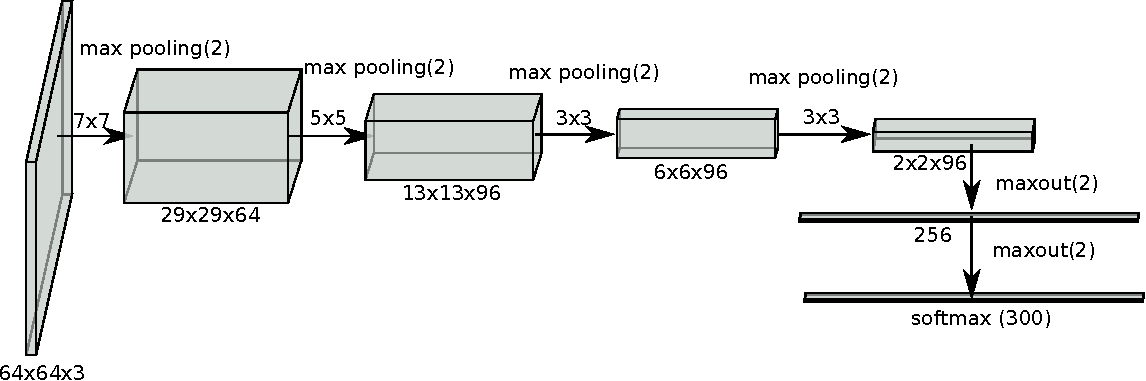
\includegraphics[width=1\textwidth]{convnet.pdf}
\caption{Convolutional network configuration used for $64\times64$ rgb images with supervised learning.}
\label{fig:convnet}
\end{figure}

We used a fairly standard convolutional neural network of six layers, with four layers of convolution and max pooling using rectified linear activation functions, two fully connected layers using maxout \cite{Springenberg2013} units as an activation method, shown in Figure~\ref{fig:convnet}. Dropout \cite{HintonDropout} with a rate of $ 0.5 $ is used when training on inputs to the two fully connected layers. For metric learning, the last linear layer and softmax are removed, leaving four convolutional layers and a single fully connected layer giving descriptors of size $ 256 $.

Dropout and Maxout have been shown to be beneficial in a supervised learning scenario for the purposes regularization. In the standard supervised training scenario Dropout is of great practical use because it (to some degree) prevents overfitting, and mostly does away with the need for early stopping. However we found that it prevented good generalization when used with metric learning approaches.

\subsection {Data augmentation}

\begin{figure}[h]
\centering
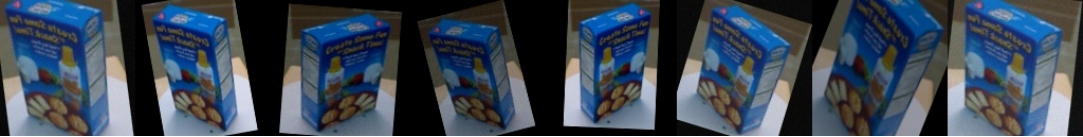
\includegraphics[width=1\textwidth]{augmentation.png}
\caption{Example of image distortions resulting from transformations of a single source image}
\label{fig:augmentation}
\end{figure}


In all cases we used randomized data augmentation of the test set by applying random distortions to ensure the network never saw exactly the same image twice, and to increase its tolerance to small changes in lighting, translation and rotation. The parameters of the data augmenmtation can be seen in Figure \ref{fig:permute}. Without the data augmenmtation supervised training produces substantially worse generalization than without in both supervised and metric learning approaches. In all experiments testing was performed on non-distorted images and trained with distorted images.

\begin{table*}
  \centering
    \caption{Ranges of parameters used for image distortion }

  \begin{tabular}{ l  l }
    \toprule
    scale (uniform) & $ 1 \pm 0.2 $  \\ 
    squash  & $ 1 \pm 0.2 $  \\ 
    rotation (rads) & $ \pm \frac{\pi}{16} $ \\ 
    translation(x, y) (\% image size) & $ \pm 5 \% $ \\ 
    brightness (additive) & $ \pm 20 \% $ \\ 
    contrast (multiplicative) & $ 1 \pm 0.2 \% $ \\ 
    gaussian pixel noise & $ \sigma = 2 \pm 2 $  \\ 
    flip horizontal (probability) & $ 0.5 $ \\ 
    \bottomrule
  \end{tabular}
\label{fig:permute}
\end{table*}

\subsection {Dataset}

\begin{figure}[h]
\centering
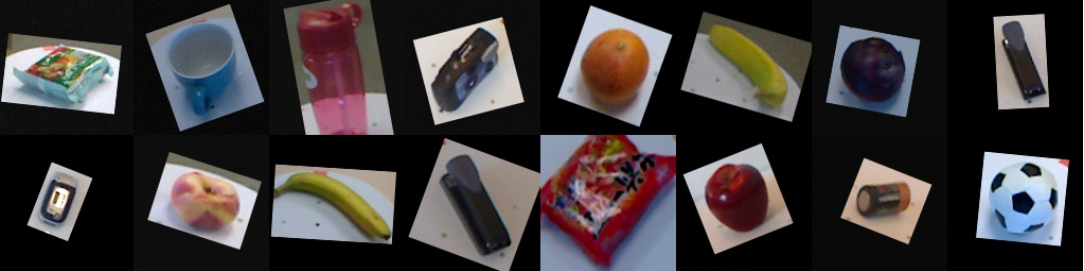
\includegraphics[width=1\textwidth]{objects.png}
\caption{Example of image distortions resulting from transformations of a single source image}
\label{fig:dataset}
\end{figure}

We experimented with the University of Washington RGB-D dataset primarily because it has a standard test set for instance recongition and a large number of published results, it contains 300 objects from 50 classes. Each object has 3 sequences of rotations at 30, 45 and 60 degrees elevation, each rotation sequence contains approximately 150 images. For instance recognition the sequence at 30 and 60 degrees are used for training and the sequence at 45 degrees is used for testing. 

We used a cut down version of the RGB-D dataset for a number of experiments, with 50 objects and 100 images of each object to train on, and 50 images per object to test. The images were randomly selected.

We used a resolution of $ 64\times64 $ on the RGB-D images, we used the cropped version of the data, our proceedure for resizing was to load all of the images in a sequence and if any image was at a higher resolution than $ 72\times72 $ we resized the image to $ 72\times72 $ and all other images in the sequence by the same ratio. The images were then distorted (see Figure~\ref{fig:permute}) and finally centered (modulo translation) on a  $ 64\times64 $ with a black background.


\section {Experiments}


In all cases (unless otherwise specified) we use a minibatch size of 256, with standard \gls{SGD} learning rate set to $ 10^{-2} $ for supervised learning, and $ 10^{-5} $ for metric learning methods. We experimented with other learning rates for metric learning, in some cases a lower learning rate of $ 10^{-6} $ was used when the higher rate caused divergence.

We manually divided the training rate by a factor of 10 when the training set accuracy plateaus for supervised learning. Supervised learning methods greatly benefit from reducing the learning rate after time, however we did not notice any benefit to the metric learning methods. Metric learning methods we stopped at 70 epochs, or earlier if they were not converging. Overall we found \gls{MEGM} to give similar, but slightly better test set accuracy than \gls{NCA}, we performed most experiments with \gls{MEGM} for consistency.



\subsection{Overall Comparison}

We compare the testing classification error between methods, the final accuracy
is reported as the test set classification accuracy average over the last 5 iterations.
Test set accuracy is percentage accuracy for supervised learning, and for metric
learning by $k = 5$ nearest neighbours and selecting the most common class.




\begin{table*}[ht]

\centering
  \caption{Summary of training methods}

  \begin{tabular}{  l l  l  l l l }
  
    \toprule
    Method &  Sampling & Batch  & Test accuracy &  Train epochs \\  \hline
    \bf{Initialization} & &  &  $ 64.0  $ & 0  &  \\  
    \hline
    
    \bf{Supervised} & & 256 &  $ 90.6  $ & 40  &  \\  
     & 5NN  &  &  $ 89.0  $ & 40 &  \\  
     \hline
    
    \bf{NCA} &  & batch &  $  71.2  $ &  50  & \\
     & random & 256 & $  94.0  $ & 70 & \\
    
    \hline
    
    \bf{MEGM} &  & batch  &  $  74.4  $ &  50  & \\
     & random & 128 &  $  95.0  $ &  70  & \\     
     &  & 256 & $  90.5  $ &  70 & \\  
     &  & 512 & $  81.4  $ &  70 & \\
    
    \hline
    \bf{MEGM} & stratified & 128 & $  {\bf 95.4 }  $ & 70 & \\  
    
     &  & 256 & $  94.6  $ & 70 & \\  
     &  & 512 & $  87.1  $ & 70 & \\  

     \hline
     
    \bf{MEGM} & neighbourhoods & 256 & $  80.4  $ & 70  & \\
    
    \hline
    
    \bf{MEGM + MSE} & stratified & 128 & $  {\bf 95.3 }  $ & 70  & \\

      \bottomrule
    
    \end{tabular}
\label{fig:summary}
\end{table*}



We sought to compare the sampling approximation to the batch method.
As a batch method, clearly \gls{SGD} is not the ideal training method. We were
surprised to see that despite the loss function smoothly decreasing (as can be
seen in Figure~\ref{fig:megm_test}), training failed to generalize well to the training set Figure~\ref{fig:megm_loss}.
We anticipated the batch metric learning methods would work best as batch
methods or with larger batches (as closer approximations to the batch method).
We can see that is not the case, and both the batch method and \gls{SGD} with the
larger batch size (512) both failed to generalize well. The same pattern occurred
for \gls{NCA}, as well as using the stratified sampling method.
The reason for such overfitting is that we believe the two metric learning
methods to have not enough bias to force the network to learn something. \gls{NCA}
allows highly complex and multi-modal distributions with many local minima
which, provided the local neighbourhood structure fits, are not penalized by it’s
loss function. Smaller batch sizes however act as a regularization, forcing the
descriptors outputs to a simpler form.



\begin{figure}[ht]
   \begin{tikzpicture}[gnuplot]
%% generated with GNUPLOT 4.6p1 (Lua 5.1; terminal rev. 99, script rev. 100)
%% Thu 31 Jul 2014 02:53:39 NZST
\gpsolidlines
\path (0.000,0.000) rectangle (12.700,7.620);
\gpcolor{color=gp lt color axes}
\gpsetlinetype{gp lt axes}
\gpsetlinewidth{1.00}
\draw[gp path] (1.504,0.985)--(12.147,0.985);
\gpcolor{color=gp lt color border}
\gpsetlinetype{gp lt border}
\draw[gp path] (1.504,0.985)--(1.684,0.985);
\draw[gp path] (12.147,0.985)--(11.967,0.985);
\node[gp node right] at (1.320,0.985) { 0};
\gpcolor{color=gp lt color axes}
\gpsetlinetype{gp lt axes}
\draw[gp path] (1.504,1.556)--(12.147,1.556);
\gpcolor{color=gp lt color border}
\gpsetlinetype{gp lt border}
\draw[gp path] (1.504,1.556)--(1.684,1.556);
\draw[gp path] (12.147,1.556)--(11.967,1.556);
\node[gp node right] at (1.320,1.556) { 0.1};
\gpcolor{color=gp lt color axes}
\gpsetlinetype{gp lt axes}
\draw[gp path] (1.504,2.127)--(12.147,2.127);
\gpcolor{color=gp lt color border}
\gpsetlinetype{gp lt border}
\draw[gp path] (1.504,2.127)--(1.684,2.127);
\draw[gp path] (12.147,2.127)--(11.967,2.127);
\node[gp node right] at (1.320,2.127) { 0.2};
\gpcolor{color=gp lt color axes}
\gpsetlinetype{gp lt axes}
\draw[gp path] (1.504,2.698)--(12.147,2.698);
\gpcolor{color=gp lt color border}
\gpsetlinetype{gp lt border}
\draw[gp path] (1.504,2.698)--(1.684,2.698);
\draw[gp path] (12.147,2.698)--(11.967,2.698);
\node[gp node right] at (1.320,2.698) { 0.3};
\gpcolor{color=gp lt color axes}
\gpsetlinetype{gp lt axes}
\draw[gp path] (1.504,3.269)--(12.147,3.269);
\gpcolor{color=gp lt color border}
\gpsetlinetype{gp lt border}
\draw[gp path] (1.504,3.269)--(1.684,3.269);
\draw[gp path] (12.147,3.269)--(11.967,3.269);
\node[gp node right] at (1.320,3.269) { 0.4};
\gpcolor{color=gp lt color axes}
\gpsetlinetype{gp lt axes}
\draw[gp path] (1.504,3.840)--(12.147,3.840);
\gpcolor{color=gp lt color border}
\gpsetlinetype{gp lt border}
\draw[gp path] (1.504,3.840)--(1.684,3.840);
\draw[gp path] (12.147,3.840)--(11.967,3.840);
\node[gp node right] at (1.320,3.840) { 0.5};
\gpcolor{color=gp lt color axes}
\gpsetlinetype{gp lt axes}
\draw[gp path] (1.504,4.411)--(12.147,4.411);
\gpcolor{color=gp lt color border}
\gpsetlinetype{gp lt border}
\draw[gp path] (1.504,4.411)--(1.684,4.411);
\draw[gp path] (12.147,4.411)--(11.967,4.411);
\node[gp node right] at (1.320,4.411) { 0.6};
\gpcolor{color=gp lt color axes}
\gpsetlinetype{gp lt axes}
\draw[gp path] (1.504,4.982)--(12.147,4.982);
\gpcolor{color=gp lt color border}
\gpsetlinetype{gp lt border}
\draw[gp path] (1.504,4.982)--(1.684,4.982);
\draw[gp path] (12.147,4.982)--(11.967,4.982);
\node[gp node right] at (1.320,4.982) { 0.7};
\gpcolor{color=gp lt color axes}
\gpsetlinetype{gp lt axes}
\draw[gp path] (1.504,5.553)--(9.759,5.553);
\draw[gp path] (11.963,5.553)--(12.147,5.553);
\gpcolor{color=gp lt color border}
\gpsetlinetype{gp lt border}
\draw[gp path] (1.504,5.553)--(1.684,5.553);
\draw[gp path] (12.147,5.553)--(11.967,5.553);
\node[gp node right] at (1.320,5.553) { 0.8};
\gpcolor{color=gp lt color axes}
\gpsetlinetype{gp lt axes}
\draw[gp path] (1.504,6.124)--(9.759,6.124);
\draw[gp path] (11.963,6.124)--(12.147,6.124);
\gpcolor{color=gp lt color border}
\gpsetlinetype{gp lt border}
\draw[gp path] (1.504,6.124)--(1.684,6.124);
\draw[gp path] (12.147,6.124)--(11.967,6.124);
\node[gp node right] at (1.320,6.124) { 0.9};
\gpcolor{color=gp lt color axes}
\gpsetlinetype{gp lt axes}
\draw[gp path] (1.504,6.695)--(12.147,6.695);
\gpcolor{color=gp lt color border}
\gpsetlinetype{gp lt border}
\draw[gp path] (1.504,6.695)--(1.684,6.695);
\draw[gp path] (12.147,6.695)--(11.967,6.695);
\node[gp node right] at (1.320,6.695) { 1};
\gpcolor{color=gp lt color axes}
\gpsetlinetype{gp lt axes}
\draw[gp path] (1.504,0.985)--(1.504,6.695);
\gpcolor{color=gp lt color border}
\gpsetlinetype{gp lt border}
\draw[gp path] (1.504,0.985)--(1.504,1.165);
\draw[gp path] (1.504,6.695)--(1.504,6.515);
\node[gp node center] at (1.504,0.677) { 0};
\gpcolor{color=gp lt color axes}
\gpsetlinetype{gp lt axes}
\draw[gp path] (3.024,0.985)--(3.024,6.695);
\gpcolor{color=gp lt color border}
\gpsetlinetype{gp lt border}
\draw[gp path] (3.024,0.985)--(3.024,1.165);
\draw[gp path] (3.024,6.695)--(3.024,6.515);
\node[gp node center] at (3.024,0.677) { 10};
\gpcolor{color=gp lt color axes}
\gpsetlinetype{gp lt axes}
\draw[gp path] (4.545,0.985)--(4.545,6.695);
\gpcolor{color=gp lt color border}
\gpsetlinetype{gp lt border}
\draw[gp path] (4.545,0.985)--(4.545,1.165);
\draw[gp path] (4.545,6.695)--(4.545,6.515);
\node[gp node center] at (4.545,0.677) { 20};
\gpcolor{color=gp lt color axes}
\gpsetlinetype{gp lt axes}
\draw[gp path] (6.065,0.985)--(6.065,6.695);
\gpcolor{color=gp lt color border}
\gpsetlinetype{gp lt border}
\draw[gp path] (6.065,0.985)--(6.065,1.165);
\draw[gp path] (6.065,6.695)--(6.065,6.515);
\node[gp node center] at (6.065,0.677) { 30};
\gpcolor{color=gp lt color axes}
\gpsetlinetype{gp lt axes}
\draw[gp path] (7.586,0.985)--(7.586,6.695);
\gpcolor{color=gp lt color border}
\gpsetlinetype{gp lt border}
\draw[gp path] (7.586,0.985)--(7.586,1.165);
\draw[gp path] (7.586,6.695)--(7.586,6.515);
\node[gp node center] at (7.586,0.677) { 40};
\gpcolor{color=gp lt color axes}
\gpsetlinetype{gp lt axes}
\draw[gp path] (9.106,0.985)--(9.106,6.695);
\gpcolor{color=gp lt color border}
\gpsetlinetype{gp lt border}
\draw[gp path] (9.106,0.985)--(9.106,1.165);
\draw[gp path] (9.106,6.695)--(9.106,6.515);
\node[gp node center] at (9.106,0.677) { 50};
\gpcolor{color=gp lt color axes}
\gpsetlinetype{gp lt axes}
\draw[gp path] (10.627,0.985)--(10.627,5.283);
\draw[gp path] (10.627,6.515)--(10.627,6.695);
\gpcolor{color=gp lt color border}
\gpsetlinetype{gp lt border}
\draw[gp path] (10.627,0.985)--(10.627,1.165);
\draw[gp path] (10.627,6.695)--(10.627,6.515);
\node[gp node center] at (10.627,0.677) { 60};
\gpcolor{color=gp lt color axes}
\gpsetlinetype{gp lt axes}
\draw[gp path] (12.147,0.985)--(12.147,6.695);
\gpcolor{color=gp lt color border}
\gpsetlinetype{gp lt border}
\draw[gp path] (12.147,0.985)--(12.147,1.165);
\draw[gp path] (12.147,6.695)--(12.147,6.515);
\node[gp node center] at (12.147,0.677) { 70};
\draw[gp path] (1.504,6.695)--(1.504,0.985)--(12.147,0.985)--(12.147,6.695)--cycle;
\node[gp node center,rotate=-270] at (0.246,3.840) {Loss function};
\node[gp node center] at (6.825,0.215) {Epoch};
\node[gp node center] at (6.825,7.157) {Effect of batch size on training};
\node[gp node right] at (10.679,6.361) {batch};
\gpcolor{color=gp lt color 0}
\gpsetlinetype{gp lt plot 0}
\draw[gp path] (10.863,6.361)--(11.779,6.361);
\draw[gp path] (1.656,4.618)--(1.808,3.418)--(1.960,3.033)--(2.112,2.821)--(2.264,2.610)%
  --(2.416,2.426)--(2.568,2.286)--(2.720,2.213)--(2.872,2.117)--(3.024,1.984)--(3.176,1.944)%
  --(3.329,1.897)--(3.481,1.981)--(3.633,1.874)--(3.785,1.800)--(3.937,1.778)--(4.089,1.778)%
  --(4.241,1.829)--(4.393,1.621)--(4.545,1.620)--(4.697,1.603)--(4.849,1.583)--(5.001,1.610)%
  --(5.153,1.571)--(5.305,1.508)--(5.457,1.543)--(5.609,1.478)--(5.761,1.464)--(5.913,1.397)%
  --(6.065,1.392)--(6.217,1.415)--(6.369,1.428)--(6.521,1.377)--(6.673,1.339)--(6.826,1.336)%
  --(6.978,1.319)--(7.130,1.323)--(7.282,1.311)--(7.434,1.281)--(7.586,1.285)--(7.738,1.269)%
  --(7.890,1.236)--(8.042,1.239)--(8.194,1.246)--(8.346,1.220)--(8.498,1.237)--(8.650,1.234)%
  --(8.802,1.224)--(8.954,1.224)--(9.106,1.229)--(9.258,1.213)--(9.410,1.195)--(9.562,1.219)%
  --(9.714,1.183)--(9.866,1.182)--(10.018,1.178)--(10.170,1.178)--(10.322,1.180)--(10.475,1.156)%
  --(10.627,1.154)--(10.779,1.163)--(10.931,1.147)--(11.083,1.130)--(11.235,1.170)--(11.387,1.161)%
  --(11.539,1.148)--(11.691,1.148)--(11.843,1.136)--(11.995,1.138)--(12.147,1.178);
\gpcolor{color=gp lt color border}
\node[gp node right] at (10.679,6.053) {512};
\gpcolor{color=gp lt color 1}
\gpsetlinetype{gp lt plot 1}
\draw[gp path] (10.863,6.053)--(11.779,6.053);
\draw[gp path] (1.656,5.309)--(1.808,4.196)--(1.960,3.211)--(2.112,3.002)--(2.264,2.943)%
  --(2.416,2.572)--(2.568,2.593)--(2.720,2.390)--(2.872,2.548)--(3.024,2.452)--(3.176,2.414)%
  --(3.329,2.647)--(3.481,2.362)--(3.633,2.350)--(3.785,2.403)--(3.937,2.347)--(4.089,2.226)%
  --(4.241,2.214)--(4.393,1.957)--(4.545,1.999)--(4.697,1.932)--(4.849,1.826)--(5.001,1.860)%
  --(5.153,1.942)--(5.305,1.952)--(5.457,2.000)--(5.609,1.978)--(5.761,1.900)--(5.913,1.980)%
  --(6.065,2.118)--(6.217,2.145)--(6.369,1.926)--(6.521,1.853)--(6.673,1.912)--(6.826,1.888)%
  --(6.978,1.804)--(7.130,1.620)--(7.282,1.626)--(7.434,1.582)--(7.586,1.623)--(7.738,1.676)%
  --(7.890,1.607)--(8.042,1.690)--(8.194,1.609)--(8.346,1.633)--(8.498,1.652)--(8.650,1.496)%
  --(8.802,1.542)--(8.954,1.581)--(9.106,1.530);
\gpcolor{color=gp lt color border}
\node[gp node right] at (10.679,5.745) {256};
\gpcolor{color=gp lt color 2}
\gpsetlinetype{gp lt plot 2}
\draw[gp path] (10.863,5.745)--(11.779,5.745);
\draw[gp path] (1.656,4.467)--(1.808,3.418)--(1.960,3.034)--(2.112,2.795)--(2.264,2.683)%
  --(2.416,2.486)--(2.568,2.405)--(2.720,2.289)--(2.872,2.228)--(3.024,2.110)--(3.176,2.035)%
  --(3.329,1.990)--(3.481,1.969)--(3.633,2.010)--(3.785,1.904)--(3.937,1.844)--(4.089,1.816)%
  --(4.241,1.763)--(4.393,1.709)--(4.545,1.642)--(4.697,1.687)--(4.849,1.723)--(5.001,1.631)%
  --(5.153,1.654)--(5.305,1.597)--(5.457,1.640)--(5.609,1.651)--(5.761,1.586)--(5.913,1.517)%
  --(6.065,1.526)--(6.217,1.518)--(6.369,1.525)--(6.521,1.487)--(6.673,1.475)--(6.826,1.496)%
  --(6.978,1.450)--(7.130,1.421)--(7.282,1.401)--(7.434,1.448)--(7.586,1.408)--(7.738,1.382)%
  --(7.890,1.390)--(8.042,1.374)--(8.194,1.373)--(8.346,1.414)--(8.498,1.321)--(8.650,1.372)%
  --(8.802,1.323)--(8.954,1.331)--(9.106,1.332)--(9.258,1.289)--(9.410,1.283)--(9.562,1.297)%
  --(9.714,1.306)--(9.866,1.269)--(10.018,1.278)--(10.170,1.285)--(10.322,1.310)--(10.475,1.340)%
  --(10.627,1.321)--(10.779,1.287)--(10.931,1.257)--(11.083,1.269)--(11.235,1.279)--(11.387,1.272)%
  --(11.539,1.260)--(11.691,1.253)--(11.843,1.215)--(11.995,1.223)--(12.147,1.231);
\gpcolor{color=gp lt color border}
\node[gp node right] at (10.679,5.437) {128};
\gpcolor{color=gp lt color 3}
\gpsetlinetype{gp lt plot 3}
\draw[gp path] (10.863,5.437)--(11.779,5.437);
\draw[gp path] (1.656,6.572)--(1.808,6.442)--(1.960,6.047)--(2.112,5.805)--(2.264,4.617)%
  --(2.416,4.256)--(2.568,3.992)--(2.720,3.976)--(2.872,3.698)--(3.024,3.666)--(3.176,3.464)%
  --(3.329,3.415)--(3.481,3.399)--(3.633,3.232)--(3.785,3.263)--(3.937,3.247)--(4.089,3.028)%
  --(4.241,2.857)--(4.393,2.915)--(4.545,2.878)--(4.697,2.809)--(4.849,2.812)--(5.001,2.879)%
  --(5.153,2.762)--(5.305,2.641)--(5.457,2.670)--(5.609,2.569)--(5.761,2.666)--(5.913,2.492)%
  --(6.065,2.432)--(6.217,2.356)--(6.369,2.376)--(6.521,2.312)--(6.673,2.331)--(6.826,2.515)%
  --(6.978,2.388)--(7.130,2.271)--(7.282,2.293)--(7.434,2.301)--(7.586,2.211)--(7.738,2.336)%
  --(7.890,2.219)--(8.042,2.230)--(8.194,2.135)--(8.346,2.145)--(8.498,2.148)--(8.650,2.101)%
  --(8.802,2.042)--(8.954,2.068)--(9.106,2.128)--(9.258,2.040)--(9.410,2.013)--(9.562,1.977)%
  --(9.714,1.972)--(9.866,1.949)--(10.018,1.981)--(10.170,2.074)--(10.322,1.988)--(10.475,1.934)%
  --(10.627,1.890)--(10.779,1.864)--(10.931,1.879)--(11.083,1.847)--(11.235,1.878)--(11.387,1.821)%
  --(11.539,1.796)--(11.691,1.820)--(11.843,1.831)--(11.995,1.845)--(12.147,1.822);
\gpcolor{color=gp lt color border}
\gpsetlinetype{gp lt border}
\draw[gp path] (1.504,6.695)--(1.504,0.985)--(12.147,0.985)--(12.147,6.695)--cycle;
%% coordinates of the plot area
\gpdefrectangularnode{gp plot 1}{\pgfpoint{1.504cm}{0.985cm}}{\pgfpoint{12.147cm}{6.695cm}}
\end{tikzpicture}
%% gnuplot variables

   \caption{Loss function for different batch sizes, MEGM loss}
   \label {fig:megm_loss}
\end{figure}

\begin{figure}[ht]
   \begin{tikzpicture}[gnuplot]
%% generated with GNUPLOT 4.6p1 (Lua 5.1; terminal rev. 99, script rev. 100)
%% Thu 31 Jul 2014 02:53:39 NZST
\gpsolidlines
\path (0.000,0.000) rectangle (12.700,7.620);
\gpcolor{color=gp lt color axes}
\gpsetlinetype{gp lt axes}
\gpsetlinewidth{1.00}
\draw[gp path] (1.320,0.985)--(12.147,0.985);
\gpcolor{color=gp lt color border}
\gpsetlinetype{gp lt border}
\draw[gp path] (1.320,0.985)--(1.500,0.985);
\draw[gp path] (12.147,0.985)--(11.967,0.985);
\node[gp node right] at (1.136,0.985) { 0};
\gpcolor{color=gp lt color axes}
\gpsetlinetype{gp lt axes}
\draw[gp path] (1.320,1.699)--(12.147,1.699);
\gpcolor{color=gp lt color border}
\gpsetlinetype{gp lt border}
\draw[gp path] (1.320,1.699)--(1.500,1.699);
\draw[gp path] (12.147,1.699)--(11.967,1.699);
\node[gp node right] at (1.136,1.699) { 5};
\gpcolor{color=gp lt color axes}
\gpsetlinetype{gp lt axes}
\draw[gp path] (1.320,2.413)--(12.147,2.413);
\gpcolor{color=gp lt color border}
\gpsetlinetype{gp lt border}
\draw[gp path] (1.320,2.413)--(1.500,2.413);
\draw[gp path] (12.147,2.413)--(11.967,2.413);
\node[gp node right] at (1.136,2.413) { 10};
\gpcolor{color=gp lt color axes}
\gpsetlinetype{gp lt axes}
\draw[gp path] (1.320,3.126)--(12.147,3.126);
\gpcolor{color=gp lt color border}
\gpsetlinetype{gp lt border}
\draw[gp path] (1.320,3.126)--(1.500,3.126);
\draw[gp path] (12.147,3.126)--(11.967,3.126);
\node[gp node right] at (1.136,3.126) { 15};
\gpcolor{color=gp lt color axes}
\gpsetlinetype{gp lt axes}
\draw[gp path] (1.320,3.840)--(12.147,3.840);
\gpcolor{color=gp lt color border}
\gpsetlinetype{gp lt border}
\draw[gp path] (1.320,3.840)--(1.500,3.840);
\draw[gp path] (12.147,3.840)--(11.967,3.840);
\node[gp node right] at (1.136,3.840) { 20};
\gpcolor{color=gp lt color axes}
\gpsetlinetype{gp lt axes}
\draw[gp path] (1.320,4.554)--(12.147,4.554);
\gpcolor{color=gp lt color border}
\gpsetlinetype{gp lt border}
\draw[gp path] (1.320,4.554)--(1.500,4.554);
\draw[gp path] (12.147,4.554)--(11.967,4.554);
\node[gp node right] at (1.136,4.554) { 25};
\gpcolor{color=gp lt color axes}
\gpsetlinetype{gp lt axes}
\draw[gp path] (1.320,5.268)--(12.147,5.268);
\gpcolor{color=gp lt color border}
\gpsetlinetype{gp lt border}
\draw[gp path] (1.320,5.268)--(1.500,5.268);
\draw[gp path] (12.147,5.268)--(11.967,5.268);
\node[gp node right] at (1.136,5.268) { 30};
\gpcolor{color=gp lt color axes}
\gpsetlinetype{gp lt axes}
\draw[gp path] (1.320,5.981)--(9.575,5.981);
\draw[gp path] (11.963,5.981)--(12.147,5.981);
\gpcolor{color=gp lt color border}
\gpsetlinetype{gp lt border}
\draw[gp path] (1.320,5.981)--(1.500,5.981);
\draw[gp path] (12.147,5.981)--(11.967,5.981);
\node[gp node right] at (1.136,5.981) { 35};
\gpcolor{color=gp lt color axes}
\gpsetlinetype{gp lt axes}
\draw[gp path] (1.320,6.695)--(12.147,6.695);
\gpcolor{color=gp lt color border}
\gpsetlinetype{gp lt border}
\draw[gp path] (1.320,6.695)--(1.500,6.695);
\draw[gp path] (12.147,6.695)--(11.967,6.695);
\node[gp node right] at (1.136,6.695) { 40};
\gpcolor{color=gp lt color axes}
\gpsetlinetype{gp lt axes}
\draw[gp path] (1.320,0.985)--(1.320,6.695);
\gpcolor{color=gp lt color border}
\gpsetlinetype{gp lt border}
\draw[gp path] (1.320,0.985)--(1.320,1.165);
\draw[gp path] (1.320,6.695)--(1.320,6.515);
\node[gp node center] at (1.320,0.677) { 0};
\gpcolor{color=gp lt color axes}
\gpsetlinetype{gp lt axes}
\draw[gp path] (2.867,0.985)--(2.867,6.695);
\gpcolor{color=gp lt color border}
\gpsetlinetype{gp lt border}
\draw[gp path] (2.867,0.985)--(2.867,1.165);
\draw[gp path] (2.867,6.695)--(2.867,6.515);
\node[gp node center] at (2.867,0.677) { 10};
\gpcolor{color=gp lt color axes}
\gpsetlinetype{gp lt axes}
\draw[gp path] (4.413,0.985)--(4.413,6.695);
\gpcolor{color=gp lt color border}
\gpsetlinetype{gp lt border}
\draw[gp path] (4.413,0.985)--(4.413,1.165);
\draw[gp path] (4.413,6.695)--(4.413,6.515);
\node[gp node center] at (4.413,0.677) { 20};
\gpcolor{color=gp lt color axes}
\gpsetlinetype{gp lt axes}
\draw[gp path] (5.960,0.985)--(5.960,6.695);
\gpcolor{color=gp lt color border}
\gpsetlinetype{gp lt border}
\draw[gp path] (5.960,0.985)--(5.960,1.165);
\draw[gp path] (5.960,6.695)--(5.960,6.515);
\node[gp node center] at (5.960,0.677) { 30};
\gpcolor{color=gp lt color axes}
\gpsetlinetype{gp lt axes}
\draw[gp path] (7.507,0.985)--(7.507,6.695);
\gpcolor{color=gp lt color border}
\gpsetlinetype{gp lt border}
\draw[gp path] (7.507,0.985)--(7.507,1.165);
\draw[gp path] (7.507,6.695)--(7.507,6.515);
\node[gp node center] at (7.507,0.677) { 40};
\gpcolor{color=gp lt color axes}
\gpsetlinetype{gp lt axes}
\draw[gp path] (9.054,0.985)--(9.054,6.695);
\gpcolor{color=gp lt color border}
\gpsetlinetype{gp lt border}
\draw[gp path] (9.054,0.985)--(9.054,1.165);
\draw[gp path] (9.054,6.695)--(9.054,6.515);
\node[gp node center] at (9.054,0.677) { 50};
\gpcolor{color=gp lt color axes}
\gpsetlinetype{gp lt axes}
\draw[gp path] (10.600,0.985)--(10.600,5.283);
\draw[gp path] (10.600,6.515)--(10.600,6.695);
\gpcolor{color=gp lt color border}
\gpsetlinetype{gp lt border}
\draw[gp path] (10.600,0.985)--(10.600,1.165);
\draw[gp path] (10.600,6.695)--(10.600,6.515);
\node[gp node center] at (10.600,0.677) { 60};
\gpcolor{color=gp lt color axes}
\gpsetlinetype{gp lt axes}
\draw[gp path] (12.147,0.985)--(12.147,6.695);
\gpcolor{color=gp lt color border}
\gpsetlinetype{gp lt border}
\draw[gp path] (12.147,0.985)--(12.147,1.165);
\draw[gp path] (12.147,6.695)--(12.147,6.515);
\node[gp node center] at (12.147,0.677) { 70};
\draw[gp path] (1.320,6.695)--(1.320,0.985)--(12.147,0.985)--(12.147,6.695)--cycle;
\node[gp node center,rotate=-270] at (0.246,3.840) {5NN testing classification error (percent)};
\node[gp node center] at (6.733,0.215) {Epoch};
\node[gp node center] at (6.733,7.157) {Effect of batch size on testing error};
\node[gp node right] at (10.679,6.361) {batch };
\gpcolor{color=gp lt color 0}
\gpsetlinetype{gp lt plot 0}
\draw[gp path] (10.863,6.361)--(11.779,6.361);
\draw[gp path] (1.629,6.164)--(1.939,6.107)--(2.248,6.090)--(2.557,5.627)--(2.867,5.576)%
  --(3.176,5.553)--(3.485,5.679)--(3.795,6.210)--(4.104,6.215)--(4.413,6.210)--(4.723,6.449)%
  --(5.032,6.666)--(5.341,6.678)--(5.651,6.370)--(5.960,6.347)--(6.269,6.472)--(6.579,6.295)%
  --(6.888,5.741)--(7.198,6.358)--(7.507,6.301)--(7.816,6.101)--(8.126,6.187)--(8.435,6.695)%
  --(8.744,6.244)--(9.054,5.250)--(9.363,4.559)--(9.672,4.440)--(9.982,4.634)--(10.291,4.542)%
  --(10.600,4.976)--(10.910,4.959)--(11.219,4.451)--(11.528,4.554)--(11.838,4.480)--(12.147,4.736);
\gpcolor{color=gp lt color border}
\node[gp node right] at (10.679,6.053) { 512};
\gpcolor{color=gp lt color 1}
\gpsetlinetype{gp lt plot 1}
\draw[gp path] (10.863,6.053)--(11.779,6.053);
\draw[gp path] (1.629,4.177)--(1.939,5.319)--(2.248,4.742)--(2.557,3.714)--(2.867,4.017)%
  --(3.176,4.086)--(3.485,3.532)--(3.795,3.840)--(4.104,3.743)--(4.413,2.949)--(4.723,3.840)%
  --(5.032,3.103)--(5.341,3.600)--(5.651,3.360)--(5.960,3.372)--(6.269,3.497)--(6.579,3.275)%
  --(6.888,3.840)--(7.198,3.646)--(7.507,3.109)--(7.816,4.040)--(8.126,3.920)--(8.435,3.149)%
  --(8.744,3.469)--(9.054,3.606);
\gpcolor{color=gp lt color border}
\node[gp node right] at (10.679,5.745) {256};
\gpcolor{color=gp lt color 2}
\gpsetlinetype{gp lt plot 2}
\draw[gp path] (10.863,5.745)--(11.779,5.745);
\draw[gp path] (1.629,3.492)--(1.939,2.915)--(2.248,2.806)--(2.557,2.669)--(2.867,2.789)%
  --(3.176,2.515)--(3.485,2.213)--(3.795,2.230)--(4.104,2.293)--(4.413,2.053)--(4.723,2.435)%
  --(5.032,2.258)--(5.341,1.967)--(5.651,1.916)--(5.960,1.870)--(6.269,2.093)--(6.579,2.030)%
  --(6.888,2.001)--(7.198,1.893)--(7.507,1.767)--(7.816,1.870)--(8.126,1.961)--(8.435,1.990)%
  --(8.744,1.790)--(9.054,2.030)--(9.363,1.716)--(9.672,1.904)--(9.982,1.961)--(10.291,1.796)%
  --(10.600,1.767)--(10.910,1.727)--(11.219,1.847)--(11.528,1.784)--(11.838,1.796)--(12.147,1.687);
\gpcolor{color=gp lt color border}
\node[gp node right] at (10.679,5.437) {128};
\gpcolor{color=gp lt color 3}
\gpsetlinetype{gp lt plot 3}
\draw[gp path] (10.863,5.437)--(11.779,5.437);
\draw[gp path] (1.629,5.582)--(1.939,3.475)--(2.248,3.583)--(2.557,3.355)--(2.867,3.143)%
  --(3.176,2.921)--(3.485,2.430)--(3.795,2.835)--(4.104,2.527)--(4.413,2.441)--(4.723,2.418)%
  --(5.032,2.213)--(5.341,2.715)--(5.651,2.544)--(5.960,2.184)--(6.269,2.247)--(6.579,2.138)%
  --(6.888,2.281)--(7.198,1.973)--(7.507,1.670)--(7.816,1.830)--(8.126,2.064)--(8.435,1.613)%
  --(8.744,1.693)--(9.054,1.636)--(9.363,1.961)--(9.672,1.824)--(9.982,1.876)--(10.291,2.013)%
  --(10.600,1.762)--(10.910,1.784)--(11.219,1.744)--(11.528,1.625)--(11.838,1.682)--(12.147,1.693);
\gpcolor{color=gp lt color border}
\gpsetlinetype{gp lt border}
\draw[gp path] (1.320,6.695)--(1.320,0.985)--(12.147,0.985)--(12.147,6.695)--cycle;
%% coordinates of the plot area
\gpdefrectangularnode{gp plot 1}{\pgfpoint{1.320cm}{0.985cm}}{\pgfpoint{12.147cm}{6.695cm}}
\end{tikzpicture}
%% gnuplot variables

   \caption{Testing error for different batch sizes, MEGM loss}
   \label {fig:megm_test}
\end{figure}



\subsection{Sampling method}

We compared the three different sampling methods, most noticeably the k-neighbourhood sampling method did not converge well. The loss function can be seen to oscillate wildly and the does not reach a local minimum (reducing the learning rate did not help), and as can be seen in Figure~\ref{fig:summary} did not produce good generalization to the test set. Reducing the learning rate did not seem to help in this case. In the same figure the results of adding in a \gls{MSE} term to the loss function can be shown to provide a slightly faster convergence rate while reaching the same testing classification error.


\section {Conclusion}

We discovered that metric learning with \gls{NCA} and \gls{MEGM} can produce good results under the right conditions. Used as a minibatch method, they're sensitive to parameters such as the batch size. Large batch sizes caused significant overfitting,
while small batch sizes produced the best generalization, and adding MSE increased convergence rate considerably. Of the proposed sampling methods, random batches and stratified sampling worked much better than neighbourhood sampling which did not converge well.


We validated the proposed idea (at least in the small scale dataset) that
the metric learning approach can be used to produce better descriptors than
standard supervised learning, despite the toy size dataset. Nonlinear MEGM
generalized a little better than NCA on this particular dataset, with similar
properties.

We are of the opinion that when either of these metric learning methods do
not provide enough bias when combined with deep neural networks. They allow
complex (and potentially multi-modal) distributions in the output descriptors,
as long as the local neighbourhood structure matches the labelling. We believe
this prevents good generalization in our experiments when the batch sizes were
larger.

Pairwise interactions complicate the implementation and we believe contribute largely to sensitivity of the training process, so make choosing the correct
sampling method much more difficult in practice. A simpler alternative we will
investigate in future is to chose a fixed descriptor to represent each class like
Nearest Class Mean (NCM) \cite {Mensink2012a}, avoiding the pairwise interaction
as well as forcing the neural network to produce a more general metric.



\section{Appendix}
\label{sec:appendix}


 We adjusted the \gls{NCA} derivative found in \cite {Salakhutdinov2007a} to give the derivative for \gls{MEGM} output for the $ i^{th} $ training case and $ t^th $ class:


\begin{equation}
\label{eq:megm_grad}
\frac{\partial \mathcal{E}_{megm}}{\partial f(x_{ti})} = 
  -2 \bigg( \sum_{j:c_i = c_j}  m_{ti} {p_{ij} \Big( d_{ij} - \sum_z{p_{iz}d_{iz}} \Big) } \bigg) 
  +2 \bigg( \sum_{j:c_i = c_j} m_{tj}{p_{ji}d_{ji} - \sum_z{\Big( \sum_{q:c_z = c_q}{p_{zq}} \Big) m_{tz}p_{zi}d_{zi}   }} \bigg)
\end{equation}

Where $ err_{ti} $ is short hand for the partial derivative $ \hat{y_{ti}} $ with respect to \gls{MSE}, and $ d_{ij} = f(x_i) - f(x_j) $ is shorthand for the difference between the descriptor vectors. The formula differs from the \gls{NCA} derivative only by the $ err_{ti} $ term.

\begin{equation}
m_{ti} = \frac{\partial \mathcal{E}_{megm}}{\partial \hat{y_{ti}}} = -2 (y_{ti} - \hat{y_{ti}})
\label{eq:megm_partial}
\end{equation}


\bibliographystyle{splncs}
\bibliography{library}
\end{document}


\bibliographystyle{unsrt}
\bibliography{references}
\end{document}